%%%%%%%% CS 886 final project report, ICML 2026 template %%%%%%%%
\documentclass{article}

\usepackage{microtype}
\usepackage{graphicx}
\usepackage{booktabs}
\usepackage{placeins}
\usepackage{array}
\usepackage{hyperref}
\newcommand{\theHalgorithm}{\arabic{algorithm}}

% Course report: the preprint option prints the author (the review option would hide it).
\usepackage[preprint]{icml2026}

\usepackage{amsmath}
\usepackage{amssymb}
\usepackage{mathtools}
\usepackage{amsthm}
\usepackage{xcolor}
\usepackage{tikz}
\usetikzlibrary{arrows.meta,positioning,decorations.pathreplacing}
\usepackage{pgfplots}
\pgfplotsset{compat=1.17}
\usepackage[capitalize,noabbrev]{cleveref}

\definecolor{Navy}{HTML}{17324D}
\definecolor{Blue}{HTML}{245E9A}
\definecolor{Muted}{HTML}{5A6775}
\definecolor{Red}{HTML}{B03A2E}
\definecolor{SensA}{HTML}{2B2D7C}
\definecolor{SensB}{HTML}{9B3FB5}
\definecolor{SensC}{HTML}{B8860B}

\theoremstyle{plain}
\newtheorem{theorem}{Theorem}
\newtheorem{proposition}{Proposition}
\newtheorem{lemma}{Lemma}
\newtheorem{corollary}{Corollary}
\theoremstyle{definition}
\newtheorem{definition}{Definition}
\newtheorem{assumption}{Assumption}
\theoremstyle{remark}
\newtheorem{remark}{Remark}

\newcommand{\E}{\mathbb{E}}
\newcommand{\R}{\mathbb{R}}
\newcommand{\one}{\mathbf{1}}
\newcommand{\sig}{\operatorname{sig}}
\newcommand{\Var}{\operatorname{Var}}
\newcommand{\Cov}{\operatorname{Cov}}
\newcommand{\softmax}{\operatorname{softmax}}
\newcommand{\nm}{\mathrm{nm}}
\newcommand{\bdet}{\beta_{\mathrm{det}}}

\icmltitlerunning{Sum Instead of AND}
% Corresponding-author line without an email (set here so the style file is unchanged).
% To add an email instead, delete these two lines and use \icmlcorrespondingauthor{Chirag Seth}{email} below.
\makeatletter\gdef\icmlcorrespondingauthor@text{Chirag Seth}\makeatother

\begin{document}

\twocolumn[
  \icmltitle{Sum Instead of AND: Why Fault Detectors Flag Look-Alikes, \\
    and How Near-Misses Teach Attention the Conjunction}

  \begin{icmlauthorlist}
    \icmlauthor{Chirag Seth}{uw}
  \end{icmlauthorlist}
  \icmlaffiliation{uw}{Department of Management Science and Engineering, University of Waterloo, Waterloo, Ontario, Canada}
  \icmlkeywords{fault detection, attention, learning theory, hypothesis testing, conjunctions}
  \vskip 0.3in
]

\printAffiliationsAndNotice{Final project report for CS 886 (Learning Theory for Modern AI), University of Waterloo, Fall 2026. }

\begin{abstract}
Learned fault detectors are trained to separate normal operation from a target fault but are deployed against a composite null hypothesis containing every condition that shifts a proper subset of the fault's $k$ sensors. Under Gaussian per-sensor evidence, the most powerful training detector thresholds the sum of the evidence (SUM), and its alarm rate on such conditions is a closed-form function of its detection rate. For deployment, the intersection--union test (AND) is within a factor $k$ of optimal, whereas every non-negative linear detector loses all power once look-alikes reach $k/(k-1)$ times the fault strength. For softmax attention pooling over sensor tokens, the inverse temperature $\beta$ interpolates between OR, SUM and AND. The gradient of the logistic loss in $\beta$ at uniform attention is derived in closed form: normal-versus-fault data keep attention at the SUM or drive it toward an OR, whereas \emph{near-misses}, conditions that omit exactly one signature sensor, drive it toward the AND. With near-misses and the head fitted at each step, every non-negative initialisation converges to an AND, and under noise the minimiser is a soft AND with $\beta^\star=\kappa\rho+O(\rho^2)$ in the near-miss share $\rho$. In transformer detectors on synthetic and LBNL fan-coil data, near-misses reverse the sign of the learned inverse temperature and reduce alarms on two-of-three look-alikes from 0.78--0.99 to 0.11--0.20 and on unseen one-sensor look-alikes to 0.02--0.06.
\end{abstract}

\section{Introduction}\label{sec:intro}

Fault detection and diagnosis (FDD) software for building equipment raises an alarm when a known fault appears in multivariate sensor data \citep{katipamula2005a,kim2018}; faults and degraded operation account for an estimated 15--30\% of commercial-building energy use \citep{katipamula2005b}. A fault shifts a characteristic set of sensors jointly, its \emph{signature}. Rule-based FDD encodes the signature as a conjunction of symptoms \citep{house2001}, but each rule requires thresholds tuned to the fault and the unit, and such rules raise many false alarms in practice \citep{andersen2024}. Learned detectors, and in particular transformers with one token per sensor, are instead trained on labelled normal and faulty windows, which are usually simulated \citep{zhao2019,granderson2023}.

Such a detector is trained to separate normal operation from one target fault, Fault~1, and is deployed against every other condition that shifts part of the signature. On the LBNL fan-coil benchmark \citep{granderson2023}, a sensor-token transformer detects a fan-outlet blockage, which shifts three sensors, in every window at a 1\% false-alarm rate, yet it raises alarms on 99\% of windows in which two of the three sensors shift, 96\% in which one shifts and 99.8\% in which one shifts strongly; the conjunction of the three symptoms raises 33\%, 8\% and 7\%. These conditions are called \emph{look-alikes} (\cref{fig:windows}).

\begin{figure}[t]
  \centering
  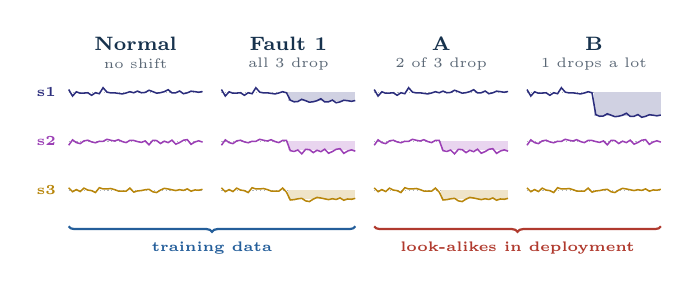
\begin{tikzpicture}
\node[font=\scriptsize\bfseries,color=Navy] at (14.50mm,6.20mm) {Normal};
\node[font=\tiny,color=Muted] at (14.50mm,3.60mm) {no shift};
\draw[Muted!50,densely dotted] (6.00mm,0.00mm)--(23.00mm,0.00mm);
\draw[SensA,line width=0.55pt] (6.00mm,0.37mm) -- (6.49mm,-0.46mm) -- (6.97mm,0.08mm) -- (7.46mm,-0.10mm) -- (7.94mm,-0.08mm) -- (8.43mm,-0.04mm) -- (8.91mm,-0.36mm) -- (9.40mm,-0.04mm) -- (9.89mm,-0.16mm) -- (10.37mm,0.60mm) -- (10.86mm,0.04mm) -- (11.34mm,-0.06mm) -- (11.83mm,-0.05mm) -- (12.31mm,-0.12mm) -- (12.80mm,-0.19mm) -- (13.29mm,-0.07mm) -- (13.77mm,0.09mm) -- (14.26mm,-0.04mm) -- (14.74mm,0.17mm) -- (15.23mm,-0.04mm) -- (15.71mm,0.00mm) -- (16.20mm,0.28mm) -- (16.69mm,0.10mm) -- (17.17mm,-0.09mm) -- (17.66mm,-0.03mm) -- (18.14mm,0.10mm) -- (18.63mm,0.35mm) -- (19.11mm,-0.05mm) -- (19.60mm,-0.04mm) -- (20.09mm,0.18mm) -- (20.57mm,-0.16mm) -- (21.06mm,-0.05mm) -- (21.54mm,0.16mm) -- (22.03mm,0.10mm) -- (22.51mm,0.02mm) -- (23.00mm,0.12mm);
\draw[Muted!50,densely dotted] (6.00mm,-6.20mm)--(23.00mm,-6.20mm);
\draw[SensB,line width=0.55pt] (6.00mm,-6.71mm) -- (6.49mm,-6.02mm) -- (6.97mm,-6.37mm) -- (7.46mm,-6.50mm) -- (7.94mm,-6.15mm) -- (8.43mm,-6.07mm) -- (8.91mm,-6.28mm) -- (9.40mm,-6.39mm) -- (9.89mm,-6.20mm) -- (10.37mm,-6.21mm) -- (10.86mm,-5.95mm) -- (11.34mm,-6.07mm) -- (11.83mm,-6.17mm) -- (12.31mm,-6.00mm) -- (12.80mm,-6.24mm) -- (13.29mm,-6.37mm) -- (13.77mm,-6.09mm) -- (14.26mm,-6.10mm) -- (14.74mm,-6.24mm) -- (15.23mm,-6.34mm) -- (15.71mm,-6.16mm) -- (16.20mm,-6.65mm) -- (16.69mm,-6.08mm) -- (17.17mm,-6.11mm) -- (17.66mm,-6.49mm) -- (18.14mm,-6.19mm) -- (18.63mm,-6.37mm) -- (19.11mm,-6.06mm) -- (19.60mm,-6.57mm) -- (20.09mm,-6.36mm) -- (20.57mm,-6.07mm) -- (21.06mm,-5.99mm) -- (21.54mm,-6.59mm) -- (22.03mm,-6.29mm) -- (22.51mm,-6.14mm) -- (23.00mm,-6.31mm);
\draw[Muted!50,densely dotted] (6.00mm,-12.40mm)--(23.00mm,-12.40mm);
\draw[SensC,line width=0.55pt] (6.00mm,-12.11mm) -- (6.49mm,-12.61mm) -- (6.97mm,-12.34mm) -- (7.46mm,-12.59mm) -- (7.94mm,-12.15mm) -- (8.43mm,-12.40mm) -- (8.91mm,-12.47mm) -- (9.40mm,-12.71mm) -- (9.89mm,-12.10mm) -- (10.37mm,-12.26mm) -- (10.86mm,-12.26mm) -- (11.34mm,-12.20mm) -- (11.83mm,-12.34mm) -- (12.31mm,-12.52mm) -- (12.80mm,-12.54mm) -- (13.29mm,-12.54mm) -- (13.77mm,-12.15mm) -- (14.26mm,-12.66mm) -- (14.74mm,-12.51mm) -- (15.23mm,-12.46mm) -- (15.71mm,-12.36mm) -- (16.20mm,-12.30mm) -- (16.69mm,-12.62mm) -- (17.17mm,-12.71mm) -- (17.66mm,-12.40mm) -- (18.14mm,-12.18mm) -- (18.63mm,-12.26mm) -- (19.11mm,-12.36mm) -- (19.60mm,-12.46mm) -- (20.09mm,-12.35mm) -- (20.57mm,-12.44mm) -- (21.06mm,-12.25mm) -- (21.54mm,-12.54mm) -- (22.03mm,-12.38mm) -- (22.51mm,-12.42mm) -- (23.00mm,-12.30mm);
\node[font=\scriptsize\bfseries,color=Navy] at (33.90mm,6.20mm) {Fault 1};
\node[font=\tiny,color=Muted] at (33.90mm,3.60mm) {all 3 drop};
\draw[Muted!50,densely dotted] (25.40mm,0.00mm)--(42.40mm,0.00mm);
\fill[SensA!22] (33.90mm,0.00mm) rectangle (42.40mm,-1.15mm);
\draw[SensA,line width=0.55pt] (25.40mm,0.37mm) -- (25.89mm,-0.46mm) -- (26.37mm,0.08mm) -- (26.86mm,-0.10mm) -- (27.34mm,-0.08mm) -- (27.83mm,-0.04mm) -- (28.31mm,-0.36mm) -- (28.80mm,-0.04mm) -- (29.29mm,-0.16mm) -- (29.77mm,0.60mm) -- (30.26mm,0.04mm) -- (30.74mm,-0.06mm) -- (31.23mm,-0.05mm) -- (31.71mm,-0.12mm) -- (32.20mm,-0.19mm) -- (32.69mm,-0.07mm) -- (33.17mm,0.09mm) -- (33.66mm,-0.04mm) -- (34.14mm,-0.98mm) -- (34.63mm,-1.19mm) -- (35.11mm,-1.15mm) -- (35.60mm,-0.87mm) -- (36.09mm,-1.05mm) -- (36.57mm,-1.24mm) -- (37.06mm,-1.18mm) -- (37.54mm,-1.05mm) -- (38.03mm,-0.80mm) -- (38.51mm,-1.20mm) -- (39.00mm,-1.19mm) -- (39.49mm,-0.97mm) -- (39.97mm,-1.31mm) -- (40.46mm,-1.20mm) -- (40.94mm,-0.99mm) -- (41.43mm,-1.05mm) -- (41.91mm,-1.13mm) -- (42.40mm,-1.03mm);
\draw[Muted!50,densely dotted] (25.40mm,-6.20mm)--(42.40mm,-6.20mm);
\fill[SensB!22] (33.90mm,-6.20mm) rectangle (42.40mm,-7.35mm);
\draw[SensB,line width=0.55pt] (25.40mm,-6.71mm) -- (25.89mm,-6.02mm) -- (26.37mm,-6.37mm) -- (26.86mm,-6.50mm) -- (27.34mm,-6.15mm) -- (27.83mm,-6.07mm) -- (28.31mm,-6.28mm) -- (28.80mm,-6.39mm) -- (29.29mm,-6.20mm) -- (29.77mm,-6.21mm) -- (30.26mm,-5.95mm) -- (30.74mm,-6.07mm) -- (31.23mm,-6.17mm) -- (31.71mm,-6.00mm) -- (32.20mm,-6.24mm) -- (32.69mm,-6.37mm) -- (33.17mm,-6.09mm) -- (33.66mm,-6.10mm) -- (34.14mm,-7.39mm) -- (34.63mm,-7.49mm) -- (35.11mm,-7.31mm) -- (35.60mm,-7.80mm) -- (36.09mm,-7.23mm) -- (36.57mm,-7.26mm) -- (37.06mm,-7.64mm) -- (37.54mm,-7.34mm) -- (38.03mm,-7.52mm) -- (38.51mm,-7.21mm) -- (39.00mm,-7.72mm) -- (39.49mm,-7.51mm) -- (39.97mm,-7.22mm) -- (40.46mm,-7.14mm) -- (40.94mm,-7.74mm) -- (41.43mm,-7.44mm) -- (41.91mm,-7.29mm) -- (42.40mm,-7.46mm);
\draw[Muted!50,densely dotted] (25.40mm,-12.40mm)--(42.40mm,-12.40mm);
\fill[SensC!22] (33.90mm,-12.40mm) rectangle (42.40mm,-13.55mm);
\draw[SensC,line width=0.55pt] (25.40mm,-12.11mm) -- (25.89mm,-12.61mm) -- (26.37mm,-12.34mm) -- (26.86mm,-12.59mm) -- (27.34mm,-12.15mm) -- (27.83mm,-12.40mm) -- (28.31mm,-12.47mm) -- (28.80mm,-12.71mm) -- (29.29mm,-12.10mm) -- (29.77mm,-12.26mm) -- (30.26mm,-12.26mm) -- (30.74mm,-12.20mm) -- (31.23mm,-12.34mm) -- (31.71mm,-12.52mm) -- (32.20mm,-12.54mm) -- (32.69mm,-12.54mm) -- (33.17mm,-12.15mm) -- (33.66mm,-12.66mm) -- (34.14mm,-13.66mm) -- (34.63mm,-13.61mm) -- (35.11mm,-13.51mm) -- (35.60mm,-13.45mm) -- (36.09mm,-13.77mm) -- (36.57mm,-13.86mm) -- (37.06mm,-13.55mm) -- (37.54mm,-13.33mm) -- (38.03mm,-13.41mm) -- (38.51mm,-13.51mm) -- (39.00mm,-13.61mm) -- (39.49mm,-13.50mm) -- (39.97mm,-13.59mm) -- (40.46mm,-13.40mm) -- (40.94mm,-13.69mm) -- (41.43mm,-13.53mm) -- (41.91mm,-13.57mm) -- (42.40mm,-13.45mm);
\node[font=\scriptsize\bfseries,color=Navy] at (53.30mm,6.20mm) {A};
\node[font=\tiny,color=Muted] at (53.30mm,3.60mm) {2 of 3 drop};
\draw[Muted!50,densely dotted] (44.80mm,0.00mm)--(61.80mm,0.00mm);
\draw[SensA,line width=0.55pt] (44.80mm,0.37mm) -- (45.29mm,-0.46mm) -- (45.77mm,0.08mm) -- (46.26mm,-0.10mm) -- (46.74mm,-0.08mm) -- (47.23mm,-0.04mm) -- (47.71mm,-0.36mm) -- (48.20mm,-0.04mm) -- (48.69mm,-0.16mm) -- (49.17mm,0.60mm) -- (49.66mm,0.04mm) -- (50.14mm,-0.06mm) -- (50.63mm,-0.05mm) -- (51.11mm,-0.12mm) -- (51.60mm,-0.19mm) -- (52.09mm,-0.07mm) -- (52.57mm,0.09mm) -- (53.06mm,-0.04mm) -- (53.54mm,0.17mm) -- (54.03mm,-0.04mm) -- (54.51mm,0.00mm) -- (55.00mm,0.28mm) -- (55.49mm,0.10mm) -- (55.97mm,-0.09mm) -- (56.46mm,-0.03mm) -- (56.94mm,0.10mm) -- (57.43mm,0.35mm) -- (57.91mm,-0.05mm) -- (58.40mm,-0.04mm) -- (58.89mm,0.18mm) -- (59.37mm,-0.16mm) -- (59.86mm,-0.05mm) -- (60.34mm,0.16mm) -- (60.83mm,0.10mm) -- (61.31mm,0.02mm) -- (61.80mm,0.12mm);
\draw[Muted!50,densely dotted] (44.80mm,-6.20mm)--(61.80mm,-6.20mm);
\fill[SensB!22] (53.30mm,-6.20mm) rectangle (61.80mm,-7.35mm);
\draw[SensB,line width=0.55pt] (44.80mm,-6.71mm) -- (45.29mm,-6.02mm) -- (45.77mm,-6.37mm) -- (46.26mm,-6.50mm) -- (46.74mm,-6.15mm) -- (47.23mm,-6.07mm) -- (47.71mm,-6.28mm) -- (48.20mm,-6.39mm) -- (48.69mm,-6.20mm) -- (49.17mm,-6.21mm) -- (49.66mm,-5.95mm) -- (50.14mm,-6.07mm) -- (50.63mm,-6.17mm) -- (51.11mm,-6.00mm) -- (51.60mm,-6.24mm) -- (52.09mm,-6.37mm) -- (52.57mm,-6.09mm) -- (53.06mm,-6.10mm) -- (53.54mm,-7.39mm) -- (54.03mm,-7.49mm) -- (54.51mm,-7.31mm) -- (55.00mm,-7.80mm) -- (55.49mm,-7.23mm) -- (55.97mm,-7.26mm) -- (56.46mm,-7.64mm) -- (56.94mm,-7.34mm) -- (57.43mm,-7.52mm) -- (57.91mm,-7.21mm) -- (58.40mm,-7.72mm) -- (58.89mm,-7.51mm) -- (59.37mm,-7.22mm) -- (59.86mm,-7.14mm) -- (60.34mm,-7.74mm) -- (60.83mm,-7.44mm) -- (61.31mm,-7.29mm) -- (61.80mm,-7.46mm);
\draw[Muted!50,densely dotted] (44.80mm,-12.40mm)--(61.80mm,-12.40mm);
\fill[SensC!22] (53.30mm,-12.40mm) rectangle (61.80mm,-13.55mm);
\draw[SensC,line width=0.55pt] (44.80mm,-12.11mm) -- (45.29mm,-12.61mm) -- (45.77mm,-12.34mm) -- (46.26mm,-12.59mm) -- (46.74mm,-12.15mm) -- (47.23mm,-12.40mm) -- (47.71mm,-12.47mm) -- (48.20mm,-12.71mm) -- (48.69mm,-12.10mm) -- (49.17mm,-12.26mm) -- (49.66mm,-12.26mm) -- (50.14mm,-12.20mm) -- (50.63mm,-12.34mm) -- (51.11mm,-12.52mm) -- (51.60mm,-12.54mm) -- (52.09mm,-12.54mm) -- (52.57mm,-12.15mm) -- (53.06mm,-12.66mm) -- (53.54mm,-13.66mm) -- (54.03mm,-13.61mm) -- (54.51mm,-13.51mm) -- (55.00mm,-13.45mm) -- (55.49mm,-13.77mm) -- (55.97mm,-13.86mm) -- (56.46mm,-13.55mm) -- (56.94mm,-13.33mm) -- (57.43mm,-13.41mm) -- (57.91mm,-13.51mm) -- (58.40mm,-13.61mm) -- (58.89mm,-13.50mm) -- (59.37mm,-13.59mm) -- (59.86mm,-13.40mm) -- (60.34mm,-13.69mm) -- (60.83mm,-13.53mm) -- (61.31mm,-13.57mm) -- (61.80mm,-13.45mm);
\node[font=\scriptsize\bfseries,color=Navy] at (72.70mm,6.20mm) {B};
\node[font=\tiny,color=Muted] at (72.70mm,3.60mm) {1 drops a lot};
\draw[Muted!50,densely dotted] (64.20mm,0.00mm)--(81.20mm,0.00mm);
\fill[SensA!22] (72.70mm,0.00mm) rectangle (81.20mm,-2.99mm);
\draw[SensA,line width=0.55pt] (64.20mm,0.37mm) -- (64.69mm,-0.46mm) -- (65.17mm,0.08mm) -- (65.66mm,-0.10mm) -- (66.14mm,-0.08mm) -- (66.63mm,-0.04mm) -- (67.11mm,-0.36mm) -- (67.60mm,-0.04mm) -- (68.09mm,-0.16mm) -- (68.57mm,0.60mm) -- (69.06mm,0.04mm) -- (69.54mm,-0.06mm) -- (70.03mm,-0.05mm) -- (70.51mm,-0.12mm) -- (71.00mm,-0.19mm) -- (71.49mm,-0.07mm) -- (71.97mm,0.09mm) -- (72.46mm,-0.04mm) -- (72.94mm,-2.82mm) -- (73.43mm,-3.03mm) -- (73.91mm,-2.99mm) -- (74.40mm,-2.71mm) -- (74.89mm,-2.89mm) -- (75.37mm,-3.08mm) -- (75.86mm,-3.02mm) -- (76.34mm,-2.89mm) -- (76.83mm,-2.64mm) -- (77.31mm,-3.04mm) -- (77.80mm,-3.03mm) -- (78.29mm,-2.81mm) -- (78.77mm,-3.15mm) -- (79.26mm,-3.04mm) -- (79.74mm,-2.83mm) -- (80.23mm,-2.89mm) -- (80.71mm,-2.97mm) -- (81.20mm,-2.87mm);
\draw[Muted!50,densely dotted] (64.20mm,-6.20mm)--(81.20mm,-6.20mm);
\draw[SensB,line width=0.55pt] (64.20mm,-6.71mm) -- (64.69mm,-6.02mm) -- (65.17mm,-6.37mm) -- (65.66mm,-6.50mm) -- (66.14mm,-6.15mm) -- (66.63mm,-6.07mm) -- (67.11mm,-6.28mm) -- (67.60mm,-6.39mm) -- (68.09mm,-6.20mm) -- (68.57mm,-6.21mm) -- (69.06mm,-5.95mm) -- (69.54mm,-6.07mm) -- (70.03mm,-6.17mm) -- (70.51mm,-6.00mm) -- (71.00mm,-6.24mm) -- (71.49mm,-6.37mm) -- (71.97mm,-6.09mm) -- (72.46mm,-6.10mm) -- (72.94mm,-6.24mm) -- (73.43mm,-6.34mm) -- (73.91mm,-6.16mm) -- (74.40mm,-6.65mm) -- (74.89mm,-6.08mm) -- (75.37mm,-6.11mm) -- (75.86mm,-6.49mm) -- (76.34mm,-6.19mm) -- (76.83mm,-6.37mm) -- (77.31mm,-6.06mm) -- (77.80mm,-6.57mm) -- (78.29mm,-6.36mm) -- (78.77mm,-6.07mm) -- (79.26mm,-5.99mm) -- (79.74mm,-6.59mm) -- (80.23mm,-6.29mm) -- (80.71mm,-6.14mm) -- (81.20mm,-6.31mm);
\draw[Muted!50,densely dotted] (64.20mm,-12.40mm)--(81.20mm,-12.40mm);
\draw[SensC,line width=0.55pt] (64.20mm,-12.11mm) -- (64.69mm,-12.61mm) -- (65.17mm,-12.34mm) -- (65.66mm,-12.59mm) -- (66.14mm,-12.15mm) -- (66.63mm,-12.40mm) -- (67.11mm,-12.47mm) -- (67.60mm,-12.71mm) -- (68.09mm,-12.10mm) -- (68.57mm,-12.26mm) -- (69.06mm,-12.26mm) -- (69.54mm,-12.20mm) -- (70.03mm,-12.34mm) -- (70.51mm,-12.52mm) -- (71.00mm,-12.54mm) -- (71.49mm,-12.54mm) -- (71.97mm,-12.15mm) -- (72.46mm,-12.66mm) -- (72.94mm,-12.51mm) -- (73.43mm,-12.46mm) -- (73.91mm,-12.36mm) -- (74.40mm,-12.30mm) -- (74.89mm,-12.62mm) -- (75.37mm,-12.71mm) -- (75.86mm,-12.40mm) -- (76.34mm,-12.18mm) -- (76.83mm,-12.26mm) -- (77.31mm,-12.36mm) -- (77.80mm,-12.46mm) -- (78.29mm,-12.35mm) -- (78.77mm,-12.44mm) -- (79.26mm,-12.25mm) -- (79.74mm,-12.54mm) -- (80.23mm,-12.38mm) -- (80.71mm,-12.42mm) -- (81.20mm,-12.30mm);
\node[anchor=east,font=\tiny\bfseries,color=SensA] at (5.60mm,0.00mm) {s1};
\node[anchor=east,font=\tiny\bfseries,color=SensB] at (5.60mm,-6.20mm) {s2};
\node[anchor=east,font=\tiny\bfseries,color=SensC] at (5.60mm,-12.40mm) {s3};
\draw[Blue,thick,decorate,decoration={brace,mirror,amplitude=2pt}] (6.00mm,-17.00mm) -- (42.40mm,-17.00mm) node[midway,below=2pt,font=\tiny\bfseries,color=Blue] {training data};
\draw[Red,thick,decorate,decoration={brace,mirror,amplitude=2pt}] (44.80mm,-17.00mm) -- (81.20mm,-17.00mm) node[midway,below=2pt,font=\tiny\bfseries,color=Red] {look-alikes in deployment};
\end{tikzpicture}

  \vspace{-2mm}
  \caption{Three sensors over a window (illustration). Training contains only Normal and Fault 1. Look-alikes A and B reproduce part of Fault~1's pattern but are different conditions.}\label{fig:windows}
  \vspace{-3mm}
\end{figure}

The failure concerns the logical form of the detector rather than its features. The training data contain only the two extremes ``no sensor shifted'' and ``all $k$ sensors shifted'', which a SUM rule (threshold the total evidence) and an AND rule (require every sensor) separate equally well; only the deployment data distinguish them. Unlike shortcut learning \citep{geirhos2020,shah2020}, every feature is causal, and the error lies in how the features are combined.

This report treats training and deployment as two hypothesis tests and analyses which rule softmax attention learns. The SUM solves the training problem, with a closed-form law for its alarm rate on look-alikes (\cref{thm:sum}), while deployment requires the AND, which no non-negative weighted sum replaces (\cref{thm:and}). Near-misses, the look-alikes that omit exactly one signature sensor, drive the inverse temperature of attention pooling toward the AND, and training from any AND-leaning initialisation ends at an AND (\cref{thm:attn}); under noise the minimiser is a soft AND (\cref{thm:soft}). Transformer detectors follow these predictions (\cref{sec:exp}), and \cref{tab:known} separates prior results from new ones.

\begin{table}[t]
  \caption{Prior results and new results. Related theory \citep{tarzanagh2023,abbe2023,bhattamishra2023} is discussed in \cref{app:related}.}\label{tab:known}
  \vspace{-1mm}
  \centering\footnotesize\setlength{\tabcolsep}{3pt}
  \begin{tabular}{@{}>{\raggedright\arraybackslash}p{0.21\columnwidth}>{\raggedright\arraybackslash}p{0.39\columnwidth}>{\raggedright\arraybackslash}p{0.34\columnwidth}@{}}
    \toprule
    Result & Known (tool or part) & New\\
    \midrule
    \cref{thm:sum} & (i) Neyman--Pearson & (ii) false-alarm law\\
    \cref{thm:and} & (a) Neyman--Pearson; (b) IU test \citep{berger1982} & (c,d) failure of sums\\
    \cref{thm:attn} & softmax calculus & $\partial_\beta L$ in closed form; (d) convergence\\
    \cref{thm:soft} & implicit function theorem & soft AND, slope $\kappa$, basin\\
    \bottomrule
  \end{tabular}
  \vspace{-3mm}
\end{table}

\section{Problem Setting}\label{sec:setup}

A window holds $T$ time steps of $C$ sensors, and Fault~1 shifts a set $S$ of $k\ge2$ sensors from an onset. Each sensor is summarised by its \emph{evidence}
\[
  a_j=\pm\,\frac{\text{mean before onset}-\text{mean after onset}}{\text{noise level of sensor }j},
\]
signed so that Fault~1 gives $a_j>0$. The theory works with $a\in\R^C$, and the experiments use raw windows (\cref{app:setup}).

\begin{assumption}[Gaussian evidence]\label{ass:gauss}
Normal: $a\sim N(0,\sigma^2I)$. Fault~1: $a\sim N(\delta\one_S,\sigma^2I)$, $\delta>0$, label $y=+1$. A \emph{look-alike} has $a\sim N(\mu,\sigma^2I)$ with $\operatorname{supp}\mu\subsetneq S$ and $0\le\mu_j\le M$, label $y=-1$. A \emph{near-miss of type $j$} is the look-alike $\mu=\delta(\one_S-e_j)$.
\end{assumption}

\begin{definition}[Valid detector]\label{def:valid}
A detector $\phi:\R^C\to\{0,1\}$ has false-alarm rate $\alpha=\Pr_0(\phi=1)$ on normal windows and detection rate $\bdet=\Pr_{\text{Fault 1}}(\phi=1)$. It is \emph{valid} if it also alarms with probability at most $\alpha$ under every look-alike.
\end{definition}

Training therefore poses the simple test ``normal or Fault~1'', and deployment the composite test ``Fault~1, or normal or any look-alike''.

\begin{definition}[Attention over sensors]\label{def:attn}
Each sensor is a token, and attention pooling gives the logits $q_aa_j+b_j$. The \emph{reduced attention model} keeps $\theta=(\beta,u,c)$ with $\beta=-q_a$, the \emph{inverse temperature} of the softmax:
\[
  f_\theta(a)=u\,m_\beta(a)+c,\quad m_\beta(a)=\textstyle\sum_{j}\softmax(-\beta a)_j\,a_j .
\]
At $\beta=0$, $m_0=\bar a$ (the SUM); $\beta\to+\infty$ gives $\min_ja_j$ (the AND); $\beta\to-\infty$ gives $\max_ja_j$ (an OR).
\end{definition}

Training minimises $L(\theta)=\E\,\ell(yf_\theta(a))$, $\ell(z)=\log(1+e^{-z})$, over normal, Fault~1 and near-miss windows with shares $\pi_0,\pi_t,\pi_\nm$. The \emph{profile loss} $G(\beta)=\min_{u,c}L(\beta,u,c)$ describes training in which the head $(u,c)$ is fitted between updates of $\beta$, and the \emph{profile flow} is $\dot\beta=-G'(\beta)$. Throughout, $\sig(z)=1/(1+e^{-z})$, $\Phi$ is the standard normal CDF and $z_\alpha=\Phi^{-1}(1-\alpha)$.

\section{Main Results}\label{sec:theory}

\begin{theorem}[Optimal training detector and false-alarm law]\label{thm:sum}
(i) If the normal and Fault~1 laws factor across sensors, the most powerful detector at any level $\alpha$ thresholds $\sum_{j\in S}\log\frac{p_{1j}}{p_{0j}}(a_j)$; under \cref{ass:gauss} it thresholds $\sum_{j\in S}a_j$.
(ii) Let a linear score $w^\top a$ have false-alarm rate $\alpha$ and detection rate $\bdet$, with Gaussian noise of any covariance. A condition with mean $h$ raises an alarm with probability
\[
  \Pr_h(\text{alarm})=\Phi\big(r\,(\Phi^{-1}(\bdet)+z_\alpha)-z_\alpha\big),
\]
where $r=w^\top h/(w^\top\delta\one_S)$ is the share of Fault~1's signal it carries.
\end{theorem}

For the SUM and a look-alike that shifts $m$ of the $k$ sensors, $r=m/k$, so the alarm rate on look-alikes increases with the detection rate. With $k=3$, $\delta/\sigma=3$ and $\alpha=1\%$, the SUM detects 0.998 of Fault~1 and flags 0.87 of two-of-three look-alikes. The proof (\cref{app:thm1}) factorises the likelihood ratio into per-sensor terms that are linear in $a_j$; in (ii), calibration fixes the threshold and the detection rate fixes the signal-to-noise ratio of the score.

\begin{theorem}[Validity ceiling and failure of sums]\label{thm:and}
(a) If $M\ge\delta$, every valid detector has $\bdet\le\Phi(\delta/\sigma-z_\alpha)$. (b) The AND test $\one\{\min_{j\in S}a_j/\sigma>z_\alpha\}$ \citep{berger1982} is valid for every $M$ and, if $M\ge\delta$, misses Fault~1 at most $k$ times as often as the best valid detector. (c) The best valid detector $\one\{w^\top a>t\}$ with $w\ge0$ has
\[
  \bdet=\Phi\Big(\frac{k\delta-(k-1)M}{\sigma\sqrt k}-z_\alpha\Big)
\]
while $M<\frac{k}{k-1}\delta$, and $\bdet\le\alpha$ once $M\ge\frac{k}{k-1}\delta$. (d) If $M=\infty$, no additive detector $\one\{\sum_j\psi_j(a_j)>t\}$ with some $\psi_j$ nondecreasing and unbounded is valid at a finite threshold.
\end{theorem}

The near-miss that omits sensor $j$ differs from Fault~1 only in $a_j$, which caps every valid detector; in (c), the worst look-alike $(M,\dots,M,0)$ has total $(k-1)M$, which reaches Fault~1's total $k\delta$ at $M=\frac{k}{k-1}\delta$ (\cref{app:thm2}). The obstruction lies in the form of the rule, so additional data cannot repair a sum.

\begin{theorem}[Inverse-temperature gradient and training dynamics]\label{thm:attn}
Let $(u^\star,c^\star)$ be the best SUM rule ($\beta=0$) and $f=u^\star\bar a+c^\star$. Then $u^\star>0$ and
\[
  \partial_\beta L\big|_{\text{SUM}}
  =u^\star\big(\pi_t\Delta_t\E_t\sig(-f)-\pi_\nm\Delta_\nm\E_\nm\sig(f)\big),
\]
where $\Delta_c=\frac1C\|\mu_c-\bar\mu_c\one\|^2$ is the spread of class $c$'s mean across sensors, $\Delta_t=\frac{\delta^2k(C-k)}{C^2}$ and $\Delta_\nm=\frac{\delta^2(k-1)(C-k+1)}{C^2}$. Hence
(a) without near-misses and with $C=k$, the SUM is the global minimiser;
(b) with near-misses and $C=k$, $\partial_\beta L<0$, so $\beta$ rises toward the AND;
(c) without near-misses and with $C>k$, $\partial_\beta L>0$, so $\beta$ falls toward an OR;
(d) with near-misses and $C=k$, the profile flow from every $\beta(0)\ge0$ satisfies $\beta(t)>0$ for $t>0$ and $\beta(t)\to\beta_\infty\in(0,+\infty]$, a soft AND ($G'(\beta_\infty)=0$) or the hard AND ($\beta_\infty=+\infty$).
\end{theorem}

Raising $\beta$ lowers a window's attention average at the rate of its spread $S^2(a)=\frac1C\sum_j(a_j-\bar a)^2$ (\cref{lem:calc}), whose conditional mean is a noise part $s_0$, common to all classes, plus $\Delta_c$ (\cref{lem:gauss}); the noise part multiplies $\partial L/\partial c=0$ and cancels. Part (d) holds because $G'(0)<0$ by (b) and a one-dimensional gradient flow cannot cross a critical point (\cref{app:thm3}).

\begin{theorem}[Soft conjunction under noise]\label{thm:soft}
Let $C=k$, $L_b=\frac12\E_0\ell(-f)+\frac12\E_t\ell(f)$ and $L(\theta;\rho)=(1-\rho)L_b+\rho\,\E_\nm\ell(-f)$. There are $\epsilon,b>0$ such that for $\rho\in[0,\epsilon)$: (i) a $C^1$ curve of strict local minimisers starts at the SUM rule $\theta_0=(0,\frac{k\delta}{\sigma^2},-\frac{k\delta^2}{2\sigma^2})$, with
\[
  \beta^\star(\rho)=\kappa\rho+O(\rho^2),\qquad
  \kappa=\frac{\delta\,\E_\nm[\sig(f_0)]}{2k\sigma^2\,\E_b[\ell''(yf_0)]},
\]
$\kappa\ge\frac{\delta}{8k\sigma^2}e^{k\delta^2/(8\sigma^2)}$ and $f_0$ the score of $\theta_0$; (ii) for $\rho>0$, $\beta^\star(\rho)$ is the only critical point of the profile loss in $(-b,b)$, and the profile flow from every $\beta(0)\in(-b,b)$ converges to it.
\end{theorem}

The numerator of $\kappa$ measures how strongly the SUM rule classifies near-misses as Fault~1, and the denominator is the curvature of the base loss. The implicit function theorem follows the minimiser, a Schur complement isolates $\beta$, and the same Schur complement is the curvature of the profile loss that gives the basin in (ii) (\cref{app:thm4}); without noise, $\beta\to\infty$ (\cref{rem:hard}).

Parts \ref{thm:attn}(d) and \ref{thm:soft}(ii) extend the analysis beyond uniform attention. With near-misses, every initialisation with $\beta(0)\ge0$ ends at an AND, never at the SUM or an OR, and for a small near-miss share every initialisation in a fixed interval $(-b,b)$, including OR-leaning ones, reaches the soft AND. Initialisations far on the OR side are discussed in \cref{rem:far}.

\section{Experiments}\label{sec:exp}

The predictions are tested on transformer detectors trained on raw windows: synthetic data (20 sensors, 48 steps; Fault~1 lowers three sensors by $2.5\sigma$) and the LBNL fan-coil unit \citep{granderson2023} (24 sensors, 48 steps of 15 minutes; Fault~1 is a fan-outlet blockage). The models (\cref{app:expdetails}) are a transformer with one token per sensor, self-attention \citep{vaswani2017} and attention pooling, and the same model without self-attention (\emph{attention pool}), which is the model of \cref{def:attn} with a learned embedding in place of the evidence. Each is trained on normal and Fault~1 windows (\emph{plain}) or with the three near-misses added (\emph{+NM}), at 1\% false alarms and with 3 seeds.

\begin{table}[t]
  \caption{Detection of Fault~1 (det.) and alarms on two-of-three look-alikes (2/3) at 1\% false alarms; mean of 3 seeds. \emph{law}: \cref{thm:sum}(ii) from each model's own detection rate. $\hat\beta$: learned inverse temperature of the attention pool.}\label{tab:main}
  \vspace{-1mm}
  \centering\footnotesize\setlength{\tabcolsep}{2.3pt}
  \begin{tabular}{@{}lccc|cc|cc|cc@{}}
    \toprule
    & \multicolumn{5}{c|}{Synthetic} & \multicolumn{4}{c}{LBNL fan-coil}\\
    & \multicolumn{3}{c|}{plain} & \multicolumn{2}{c|}{+NM} & \multicolumn{2}{c|}{plain} & \multicolumn{2}{c}{+NM}\\
    Model & det. & 2/3 & law & det. & 2/3 & det. & 2/3 & det. & 2/3\\
    \midrule
    Transformer & .93 & .78 & .59 & .88 & \textbf{.15} & 1.00 & .99 & 1.00 & \textbf{.18}\\
    Attention pool & .91 & .79 & .56 & .84 & \textbf{.11} & 1.00 & .98 & 1.00 & \textbf{.20}\\
    AND rule (oracle) & .90 & .22 & -- & .88 & .20 & 1.00 & .33 & 1.00 & .31\\
    \midrule
    $\hat\beta$ (attention pool) & \multicolumn{5}{c|}{$-1.06\ \to\ +0.70$} & \multicolumn{4}{c}{$-1.02\ \to\ +0.69$}\\
    \bottomrule
  \end{tabular}
  \vspace{-3mm}
\end{table}

After plain training both models detect Fault~1 and flag most two-of-three look-alikes (\cref{tab:main}). They lie about 0.2 above the law of \cref{thm:sum}(ii), with learned inverse temperature $\hat\beta=-1.06$: the OR regime of \cref{thm:attn}(c), since 17 of the 20 sensors lie outside the signature. With near-misses $\hat\beta$ becomes positive on both datasets, and in a near-miss window the sensor that did not shift receives 10.6 times the weight of the other two on synthetic data and at least 88 times on fan-coil data, against 0.14 and 0.01 without near-misses. Alarms on two-of-three look-alikes fall to 0.11--0.20, close to the AND oracle, and alarms on one-sensor and loud one-sensor look-alikes, which never appear in training, fall to 0.02--0.06. As the near-miss share $\rho$ grows, $\hat\beta$ increases and remains finite (\cref{fig:softand}), as \cref{thm:soft} predicts.

\section{Conclusion}\label{sec:conc}

The training data determine the logical form of a learned fault detector: normal-versus-fault data select the SUM, which no re-weighting makes valid against look-alikes, and near-misses move softmax attention to the AND. The analysis concerns a reduced attention model with Gaussian evidence and a known onset. The next steps are the full attention layer with learned queries and keys trained jointly with the head, near-misses in time for look-alikes that differ from the fault only in when the sensors shift, and validation on field data from several units.

\section*{Software and Data}
Code, configurations, reference results and the numerical checks are available at \url{https://github.com/chirag300/HVAC_Test}; the LBNL data are public \citep{granderson2023}. \Cref{app:repro} lists the commands.

\bibliography{references}
\bibliographystyle{icml2026}

\newpage
\appendix
\onecolumn
%% ======================================================================
%% Appendix (one column)
%% ======================================================================
\numberwithin{equation}{section}
\linespread{1.12}\selectfont
\setlength{\jot}{6pt}
\setlength{\parskip}{3pt}

\newcommand{\tocsec}[2]{\par\vspace{5pt}\noindent\hyperref[#1]{\textbf{\ref*{#1}\hspace{1em}#2}}\hfill\textbf{\pageref{#1}}\par}
\newcommand{\tocsub}[2]{\par\noindent\hspace*{2em}\hyperref[#1]{\ref*{#1}\hspace{1em}#2}\dotfill\pageref{#1}\par}
\newenvironment{restated}[1]{\par\medskip\noindent\textbf{#1 (restated).}\itshape\ }{\par\medskip}
\newcommand{\step}[1]{\par\medskip\noindent\textbf{#1}\ }

\section*{Appendix}

The appendix is organised as follows. \Cref{app:setup} completes the problem setting: the structure of faults and sensors, the evidence vector, the deployment null hypothesis and the attention model. \Cref{app:related} discusses related work. \Cref{app:proofs12} proves \cref{thm:sum,thm:and}, and \cref{app:proofs34} proves the two lemmas on the spread of the evidence and \cref{thm:attn,thm:soft}, including their parts on initialisations away from uniform attention. \Cref{app:expdetails,app:results,app:repro} give the implementation details, the full experimental results and the commands that reproduce them.

\vspace{6pt}
\noindent\textbf{\large Contents}
\vspace{2pt}

\tocsec{app:setup}{Problem Setting}
\tocsec{app:related}{Related Work}
\tocsec{app:proofs12}{Proofs of Theorems~\ref*{thm:sum} and~\ref*{thm:and}}
\tocsub{app:thm1}{Proof of Theorem~\ref*{thm:sum}}
\tocsub{app:thm2}{Proof of Theorem~\ref*{thm:and}}
\tocsec{app:proofs34}{Proofs for Attention}
\tocsub{app:lemmas}{Two lemmas on the spread of the evidence}
\tocsub{app:thm3}{Proof of Theorem~\ref*{thm:attn}}
\tocsub{app:thm4}{Proof of Theorem~\ref*{thm:soft}}
\tocsec{app:expdetails}{Implementation Details}
\tocsec{app:results}{Full Experimental Results}
\tocsec{app:repro}{Reproducibility}

\newpage
%% ----------------------------------------------------------------------
\section{Problem Setting}\label{app:setup}

\Cref{fig:faults} summarises the structure that the analysis assumes. Each condition of a unit shifts a set of sensors. The signature $S$ of Fault~1 overlaps the sets shifted by other faults, by sensor faults and by unusual operation, and a detector trained on normal and Fault~1 windows is deployed against all of them.

\begin{figure}[h]
  \centering
  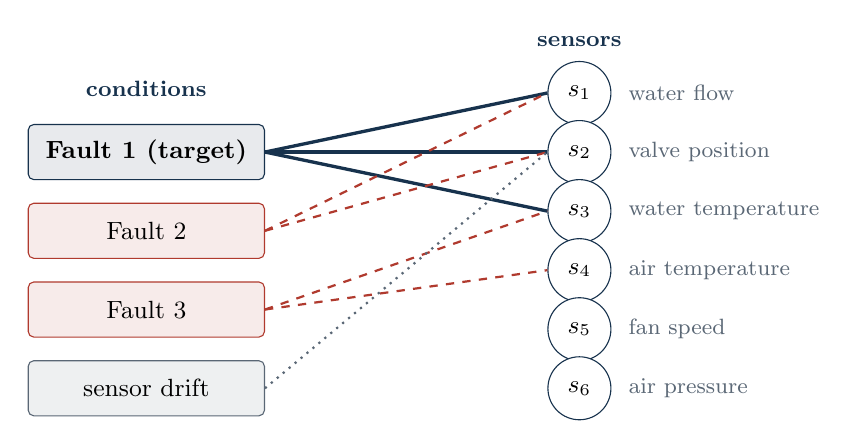
\begin{tikzpicture}[x=1mm,y=1mm,
    faultbase/.style={rounded corners=2pt,minimum width=30mm,minimum height=7mm,align=center,font=\small},
    faultN/.style={faultbase,draw=Navy,fill=Navy!10},
    faultR/.style={faultbase,draw=Red,fill=Red!10},
    faultM/.style={faultbase,draw=Muted,fill=Muted!10},
    sensor/.style={circle,draw=Navy,fill=white,minimum size=8mm,inner sep=0pt,font=\small},
    lbl/.style={font=\footnotesize,color=Muted,anchor=west}]
  % faults
  \node[faultN,font=\small\bfseries] (f1) at (0,30) {Fault 1 (target)};
  \node[faultR] (f2) at (0,20) {Fault 2};
  \node[faultR] (f3) at (0,10) {Fault 3};
  \node[faultM] (f4) at (0,0) {sensor drift};
  % sensors
  \foreach \i/\y/\name in {1/37.5/water flow,2/30/valve position,3/22.5/water temperature,4/15/air temperature,5/7.5/fan speed,6/0/air pressure}{
    \node[sensor] (s\i) at (55,\y) {$s_{\i}$};
    \node[lbl] at (60,\y) {\name};
  }
  % edges
  \foreach \s in {1,2,3}{\draw[Navy,very thick] (f1.east) -- (s\s.west);}
  \foreach \s in {1,2}{\draw[Red,thick,dashed] (f2.east) -- (s\s.west);}
  \foreach \s in {3,4}{\draw[Red,thick,dashed] (f3.east) -- (s\s.west);}
  \draw[Muted,thick,dotted] (f4.east) -- (s2.west);
  \node[font=\footnotesize\bfseries,color=Navy] at (0,38) {conditions};
  \node[font=\footnotesize\bfseries,color=Navy] at (55,44) {sensors};
\end{tikzpicture}

  \caption{Faults and sensors (illustration). Fault~1's signature is $\{s_1,s_2,s_3\}$; Fault~2, Fault~3 and a drifting sensor shift parts of it.}\label{fig:faults}
\end{figure}

A window $X\in\R^{T\times C}$ with onset $\tau$ is reduced to the evidence vector
\begin{equation}\label{eq:evidence}
  a_j \;=\; s_j\,\frac{\hat m_j^{-}-\hat m_j^{+}}{\hat\sigma_j},\qquad j=1,\dots,C,
\end{equation}
where $\hat m_j^{-}$ and $\hat m_j^{+}$ are the means of sensor $j$ before and after $\tau$, $\hat\sigma_j$ is the standard deviation of their difference under normal operation, and $s_j\in\{-1,+1\}$ is the sign under which Fault~1 increases $a_j$. As a difference of window means, $a_j$ is Gaussian when the noise is Gaussian and approximately Gaussian otherwise. It records how much a sensor shifted but not when, so look-alikes that differ from Fault~1 only in timing lie outside the scope of the theory. Under \cref{ass:gauss} the deployment null hypothesis is
\begin{equation}\label{eq:null}
  \mathcal N(M)\;=\;\big\{N(0,\sigma^2I)\big\}\ \cup\ \big\{N(\mu,\sigma^2I):\ \operatorname{supp}\mu\subsetneq S,\ 0\le\mu_j\le M\text{ for all }j\big\},
\end{equation}
and a detector is valid (\cref{def:valid}) if its alarm rate is at most $\alpha$ under every member of $\mathcal N(M)$. The members closest to Fault~1 are the near-misses $\mu^{(j)}=\delta(\one_S-e_j)$, $j\in S$, each of which differs from Fault~1 in a single coordinate.

The detector analysed in \cref{thm:attn,thm:soft} is attention pooling over sensor tokens. Token $j$ is $x_j=(a_j,e_j)\in\R^{1+C}$, the evidence together with a one-hot sensor identity, and pooling with a learned query $p$, key matrix $W$ and value vector $v$ computes
\begin{equation}\label{eq:full}
  f(a)=\sum_{j=1}^C\pi_j(a)\,x_j^\top v+c,
  \qquad
  \pi(a)=\softmax\big(x_1^\top Wp,\dots,x_C^\top Wp\big).
\end{equation}
With $Wp=(q_a,b)\in\R\times\R^C$ and $v=(u_a,u)$, the logit of token $j$ is $q_aa_j+b_j$ and its value is $u_aa_j+u_j$. The reduced model of \cref{def:attn} keeps the evidence-dependent part, $b=0$ and $u=0$, and writes $\beta=-q_a$ and $u$ for $u_a$:
\begin{equation}\label{eq:reduced}
  f_\theta(a)=u\,m_\beta(a)+c,
  \qquad
  m_\beta(a)=\sum_{j=1}^C\pi_j\,a_j,
  \qquad
  \pi_j=\frac{e^{-\beta a_j}}{\sum_{l=1}^Ce^{-\beta a_l}} .
\end{equation}
The logits are $-\beta a_j$, so $\beta$ is the inverse temperature of a soft minimum, and
\begin{equation}\label{eq:limits}
  m_0(a)=\bar a,
  \qquad
  \lim_{\beta\to+\infty}m_\beta(a)=\min_ja_j,
  \qquad
  \lim_{\beta\to-\infty}m_\beta(a)=\max_ja_j .
\end{equation}
Thresholding $f_\theta$ therefore gives the SUM rule, the AND rule and an OR rule, respectively. \Cref{rem:full} shows that at uniform attention the gradient of the full layer \cref{eq:full} has a single non-zero coordinate, the one along $q_a$, so the reduction is exact to first order there.

Training minimises the logistic loss over normal windows ($y=-1$, share $\pi_0$), Fault~1 windows ($y=+1$, share $\pi_t$) and near-misses ($y=-1$, share $\pi_\nm$, split equally over the $k$ types):
\begin{equation}\label{eq:loss}
  L(\theta)=\pi_0\,\E_0\,\ell\big(-f_\theta(a)\big)+\pi_t\,\E_t\,\ell\big(f_\theta(a)\big)+\pi_\nm\,\E_\nm\,\ell\big(-f_\theta(a)\big)=\E\,\ell\big(yf_\theta(a)\big),
\end{equation}
with $\ell'(z)=-\sig(-z)$ and $\ell''(z)=\sig(z)\sig(-z)\in(0,\tfrac14]$. Gradient descent changes $\beta$ by $-\eta\,\partial L/\partial\beta$, so the sign of $\partial L/\partial\beta$ determines whether attention moves toward the AND or toward an OR. When the head $(u,c)$ is fitted between updates of $\beta$, training follows the profile flow $\dot\beta=-G'(\beta)$ of the profile loss $G(\beta)=\min_{u,c}L(\beta,u,c)$. This is a two-timescale idealisation of joint gradient descent with the same critical points (Step~6 in \cref{app:thm3}).

\begin{center}\small
\renewcommand{\arraystretch}{1.25}
\begin{tabular}{@{}ll@{}}
\toprule
Symbol & Meaning\\
\midrule
$C$, $S$, $k=|S|$ & number of sensors; the signature of Fault~1; its size, $k\ge2$\\
$a=(a_1,\dots,a_C)$ & evidence vector, \cref{eq:evidence}\\
$\delta$, $\sigma$ & Fault~1's shift per signature sensor; noise standard deviation\\
$M$; $\mathcal N(M)$ & largest look-alike shift on one sensor; the deployment null, \cref{eq:null}\\
$\alpha$, $\bdet$ & false-alarm rate on normal windows; detection rate on Fault~1\\
$\Phi$, $\varphi$, $z_\alpha$ & standard normal CDF and density; $z_\alpha=\Phi^{-1}(1-\alpha)$, so $z_{0.01}=2.326$\\
$\bar a$, $S^2(a)$ & mean $\frac1C\sum_ja_j$ and spread $\frac1C\sum_j(a_j-\bar a)^2$ of the evidence across sensors\\
$s_0$, $\Delta(\mu)$ & noise part $\sigma^2\frac{C-1}{C}$ and pattern part $\frac1C\|\mu-\bar\mu\one\|^2$ of the expected spread\\
$\beta$; $\theta=(\beta,u,c)$ & inverse temperature; parameters of the reduced model, \cref{eq:reduced}\\
$m_\beta(a)$, $\pi(a)$ & attention-weighted average of the evidence; attention weights\\
$G(\beta)$, $(u_\beta,c_\beta)$ & profile loss $\min_{u,c}L(\beta,u,c)$; the head that attains it\\
$y$, $\ell$, $\sig$ & label ($+1$ Fault~1, $-1$ otherwise); logistic loss; sigmoid\\
$\pi_0,\pi_t,\pi_\nm$ & shares of normal, Fault~1 and near-miss windows in training\\
$\E_0,\E_t,\E_\nm$; $\E_b$ & expectation over one class; $\E_b=\frac12\E_0+\frac12\E_t$, the base mixture of \cref{thm:soft}\\
$\rho$, $\kappa$ & near-miss share in \cref{thm:soft}; slope of the optimal inverse temperature in $\rho$\\
\bottomrule
\end{tabular}
\end{center}

%% ----------------------------------------------------------------------
\section{Related Work}\label{app:related}

Fault detection and diagnosis for building systems has been surveyed extensively \citep{katipamula2005a,katipamula2005b,kim2018,zhao2019}. Rule-based systems such as the APAR rules for air-handling units \citep{house2001} encode each fault as a conjunction of symptoms, in the same way that model-based diagnosis treats a fault as a pattern of residuals \citep{gertler1998,venkat2003}. Such rules compute the AND analysed in this report, but they require thresholds tuned to every fault and every unit, and practitioners report that they raise many false alarms \citep{andersen2024}. Data-driven detectors replace the rule by a classifier trained on labelled windows, which are usually simulated; the LBNL benchmark \citep{granderson2023} provides paired faulty and fault-free simulations, from which the experiments here construct near-misses by counterfactual splicing. The question addressed in this report is which decision rule such a classifier learns from normal-versus-fault data, and which additional data change it.

A detector that fires on look-alikes resembles a model that relies on shortcuts \citep{geirhos2020,shah2020,hermann2024}. In shortcut learning a spurious feature replaces a causal one, whereas in the present setting every signature sensor is causal and the error lies in how the features are combined. This places the problem closer to work on simplicity bias. Networks trained on part of a Boolean domain converge to the minimum-degree interpolator \citep{abbe2023}, kernel models with disentangled inputs are additive across components \citep{lippl2025}, and transformers prefer functions of low sensitivity \citep{bhattamishra2023}. Each of these results predicts an additive rule after normal-versus-fault training. \Cref{thm:sum} gives a statistical reason that holds even for the Bayes-optimal detector: by the Neyman--Pearson lemma \citep{neyman1933,lehmann2005}, the sum of the evidence is the most powerful test of the training problem. The deployment problem, in contrast, is a composite test whose null hypothesis is a union of hypotheses, one for each sensor that may remain unshifted. Such problems are solved by intersection--union tests \citep{berger1982}, which reject only when every component test rejects. \Cref{thm:and}(b) applies this principle to the evidence vector, and parts (c) and (d) show that no sum can replace it.

The analysis of attention builds on recent results on how softmax attention selects and combines tokens. \citet{tarzanagh2023} show that gradient descent on softmax attention converges in direction to a max-margin solution that selects one locally optimal token per input, while the norm of the attention parameters grows without bound. \citet{wang2024} show that transformers provably learn sparse token selection where fully connected networks cannot, \citet{edelman2022} show that self-attention can represent sparse functions of its input with a sample complexity that grows only logarithmically in the context length, and \citet{hu2025} show that a single softmax attention head provably learns constrained Boolean functions. In the fault-detection setting no single token is optimal, because the signature sensors shift together, and the relevant question is how attention combines the tokens rather than which token it selects. This is governed by the inverse temperature and its sign. \Cref{thm:attn} shows that the training data decide whether attention moves toward the minimum of the evidence (AND) or toward its maximum (OR), and \cref{thm:soft} shows that under noise the inverse temperature stops at a finite value, in contrast to the norm growth that drives token selection in \citet{tarzanagh2023}. The proofs use the implicit function theorem \citep{rudin1976} to follow the minimiser as near-misses are added, and Danskin's theorem \citep{danskin1967} for the output head.

Near-misses as training examples go back to Winston's work on learning structural descriptions \citep{winston1970}, and teaching sets formalise the examples that identify a concept \citep{goldman1995}. Certifying a learned function from examples is, however, hard in general for circuits and transformers \citep{backdeluca2026}. The present report shows that for conjunctions over sensor evidence the $k$ near-misses are the examples that move softmax attention from the SUM to the AND.

%% ----------------------------------------------------------------------
\section{Proofs of Theorems~\ref*{thm:sum} and~\ref*{thm:and}}\label{app:proofs12}

\subsection{Proof of Theorem~\ref*{thm:sum}}\label{app:thm1}

\begin{restated}{Theorem~\ref{thm:sum}}
(i) Suppose that under normal operation and under Fault~1 the sensors are independent, with densities $p_0(a)=\prod_jp_{0j}(a_j)$ and $p_1(a)=\prod_jp_{1j}(a_j)$, and that $p_{1j}=p_{0j}$ for $j\notin S$. Then for every level $\alpha$ the most powerful detector of normal versus Fault~1 thresholds $\Lambda(a)=\sum_{j\in S}\log\frac{p_{1j}(a_j)}{p_{0j}(a_j)}$. Under \cref{ass:gauss} it thresholds $\sum_{j\in S}a_j$.

(ii) Let every condition have $a\sim N(h,\Sigma)$ for a common covariance $\Sigma$, and let the score $w^\top a$ satisfy $w^\top\Sigma w>0$ and $w^\top\mu_t>0$, where $\mu_t=\delta\one_S$. If the detector $\one\{w^\top a>t\}$ has false-alarm rate $\alpha$ and detection rate $\bdet$, then a condition with mean $h$ raises an alarm with probability
\begin{equation}\label{eq:law}
  \Pr_h(\text{alarm})=\Phi\Big(r_w(h)\,\big(\Phi^{-1}(\bdet)+z_\alpha\big)-z_\alpha\Big),
  \qquad
  r_w(h)=\frac{w^\top h}{w^\top\mu_t}.
\end{equation}
If $w$ is constant on $S$ and $h$ shifts $m$ of the $k$ signature sensors by $\delta$, then $r_w(h)=m/k$. For $0<r_w(h)<1$ the alarm rate increases with $\bdet$ and tends to $1$ as $\bdet\to1$.
\end{restated}

\begin{proof}
The proof of (i) takes three steps and that of (ii) four.

\step{Step 1: the most powerful detector thresholds the likelihood ratio.} The training problem tests the simple hypothesis ``normal'', with density $p_0$, against the simple hypothesis ``Fault~1'', with density $p_1$. By the Neyman--Pearson lemma \citep[Thm.~3.2.1]{neyman1933,lehmann2005}, among all detectors with false-alarm rate at most $\alpha$ the most powerful one alarms when $p_1(a)/p_0(a)$, or equivalently $\log\big(p_1(a)/p_0(a)\big)$, exceeds a threshold. The share of Fault~1 windows in the training data only moves this threshold, which calibration to level $\alpha$ fixes.

\step{Step 2: independence turns the ratio into a sum.} Both densities are products over sensors, so the logarithm of their ratio is a sum,
\begin{equation}\label{eq:llr-sum}
  \log\frac{p_1(a)}{p_0(a)}
  =\sum_{j=1}^C\log\frac{p_{1j}(a_j)}{p_{0j}(a_j)}
  =\sum_{j\in S}\log\frac{p_{1j}(a_j)}{p_{0j}(a_j)}=\Lambda(a),
\end{equation}
where the second equality holds because a sensor outside $S$ has the same density under both hypotheses. With Step~1 this proves the first claim of (i).

\step{Step 3: under Gaussian evidence each term is linear.} Under \cref{ass:gauss}, sensor $j\in S$ has density $N(0,\sigma^2)$ under normal operation and $N(\delta,\sigma^2)$ under Fault~1. The normalising constants cancel, and
\begin{equation}\label{eq:gauss-term}
  \log\frac{p_{1j}(a_j)}{p_{0j}(a_j)}
  =\frac{a_j^2-(a_j-\delta)^2}{2\sigma^2}
  =\frac{\delta}{\sigma^2}\,a_j-\frac{\delta^2}{2\sigma^2}.
\end{equation}
Summing over the $k$ sensors of $S$,
\begin{equation}\label{eq:gauss-llr}
  \boxed{\;\Lambda(a)=\frac{\delta}{\sigma^2}\sum_{j\in S}a_j-\frac{k\delta^2}{2\sigma^2}.\;}
\end{equation}
Since $\delta/\sigma^2>0$, the event $\{\Lambda(a)>t\}$ equals $\{\sum_{j\in S}a_j>t'\}$ with $t'=\frac{\sigma^2}{\delta}\big(t+\frac{k\delta^2}{2\sigma^2}\big)$, so the most powerful detector is the SUM rule. This proves (i).

\step{Step 4: the score of every condition is Gaussian.} Fix $w$ and let $s_w=\sqrt{w^\top\Sigma w}>0$. Under a condition with mean $h$,
\begin{equation}\label{eq:score-law}
  w^\top a\sim N\big(w^\top h,\ s_w^2\big).
\end{equation}

\step{Step 5: the false-alarm rate fixes the threshold.} Normal windows have $h=0$, and the condition $\Pr_0(w^\top a>t)=1-\Phi(t/s_w)=\alpha$ gives
\begin{equation}\label{eq:threshold}
  t=z_\alpha\,s_w .
\end{equation}

\step{Step 6: the detection rate fixes the signal-to-noise ratio.} Let $D_w=w^\top\mu_t/s_w$. By \cref{eq:score-law,eq:threshold} with $h=\mu_t$,
\begin{equation}\label{eq:snr}
  \bdet=\Pr_{\mu_t}(w^\top a>t)
  =\Phi\big(D_w-z_\alpha\big),
  \qquad\text{so}\qquad
  D_w=\Phi^{-1}(\bdet)+z_\alpha .
\end{equation}

\step{Step 7: every other condition lies a fraction $r_w(h)$ of the way.} For a condition with mean $h$, the same computation gives
\begin{equation}\label{eq:other}
  \Pr_h(w^\top a>t)
  =\Phi\Big(\frac{w^\top h}{s_w}-z_\alpha\Big)
  =\Phi\big(r_w(h)\,D_w-z_\alpha\big),
\end{equation}
and substituting $D_w$ from \cref{eq:snr},
\begin{equation}\label{eq:law-proof}
  \boxed{\;\Pr_h(\text{alarm})=\Phi\Big(r_w(h)\,\big(\Phi^{-1}(\bdet)+z_\alpha\big)-z_\alpha\Big).\;}
\end{equation}
If $w_j=w_S$ for every $j\in S$ and $h$ equals $\delta$ on $m$ coordinates of $S$ and $0$ elsewhere, then $w^\top h=m\delta w_S$ and $w^\top\mu_t=k\delta w_S$, so $r_w(h)=m/k$. Finally, $\Phi^{-1}$ is increasing and tends to $+\infty$ at $1$, so for $r_w(h)>0$ the argument in \cref{eq:law-proof} increases with $\bdet$ and tends to $+\infty$.
\end{proof}

\subsection{Proof of Theorem~\ref*{thm:and}}\label{app:thm2}

The proof is restricted to the $k$ signature sensors, so that Fault~1 has mean $\delta\one$ and the null hypothesis is $\mathcal N(M)$ of \cref{eq:null}. Sensors outside $S$ have the same law in every class; part (a) holds with them included because its argument uses one coordinate, and in parts (b)--(d) a positive weight on them only adds noise to the score.

\begin{restated}{Theorem~\ref{thm:and}}
(a) If $M\ge\delta$, every valid detector has $\bdet\le\Phi(\delta/\sigma-z_\alpha)$.
(b) The AND test $\phi_{\mathrm{AND}}(a)=\one\{\min_ja_j/\sigma>z_\alpha\}$ is valid for every $M$, and its detection rate is $\Phi(\delta/\sigma-z_\alpha)^k$. If $M\ge\delta$, it misses Fault~1 at most $k$ times as often as the best valid detector.
(c) For every $M\ge0$, the best valid detector of the form $\one\{w^\top a>t\}$ with $w\ge0$, $w\neq0$, has detection rate $\Phi\big(\frac{k\delta-(k-1)M}{\sigma\sqrt k}-z_\alpha\big)$, attained at $w=\one$, as long as $M<\frac{k}{k-1}\delta$. Once $M\ge\frac{k}{k-1}\delta$, every valid detector of this form has detection rate at most $\alpha$.
(d) If $M=\infty$, every additive detector $\one\{\sum_j\psi_j(a_j)>t\}$ with finite-valued $\psi_j$, at least one of which is nondecreasing and unbounded above, has alarm rate tending to $1$ along single-sensor look-alikes. It is valid only with $t=+\infty$, that is, with detection rate $0$.
\end{restated}

\begin{proof}
\step{Part (a): one near-miss caps every valid detector.} Fix a sensor $j$. Since $M\ge\delta$, the near-miss $\mu^{(j)}=\delta(\one-e_j)$ belongs to $\mathcal N(M)$, so a valid detector is a level-$\alpha$ test of $N(\mu^{(j)},\sigma^2I)$ against $N(\delta\one,\sigma^2I)$. The two laws agree on every coordinate except $j$, where the means are $0$ and $\delta$, and their likelihood ratio
\begin{equation}\label{eq:nm-ratio}
  \frac{\varphi\big((a_j-\delta)/\sigma\big)}{\varphi\big(a_j/\sigma\big)}
  =\exp\Big(\frac{\delta}{\sigma^2}a_j-\frac{\delta^2}{2\sigma^2}\Big)
\end{equation}
is a function of $a_j$ alone that increases in $a_j$. By the Neyman--Pearson lemma the most powerful level-$\alpha$ test of this pair alarms when $a_j>z_\alpha\sigma$, with power
\begin{equation}\label{eq:ceiling}
  \boxed{\;\Pr_{\delta\one}\big(a_j>z_\alpha\sigma\big)=\Phi\big(\delta/\sigma-z_\alpha\big).\;}
\end{equation}
No valid detector does better against this pair, and hence none does better against $\mathcal N(M)$.

\step{Part (b), validity.} Every member of $\mathcal N(M)$ has a sensor $j$ with $\mu_j=0$, and the AND test alarms only if this sensor passes its own test:
\begin{equation}\label{eq:and-valid}
  \boxed{\;\Pr_\mu\big(\phi_{\mathrm{AND}}=1\big)
  \le\Pr_\mu\big(a_j>z_\alpha\sigma\big)
  =1-\Phi(z_\alpha)=\alpha .\;}
\end{equation}
This holds for every $M$, including $M=\infty$; it is the intersection--union principle \citep{berger1982} applied to the hypotheses ``sensor $j$ did not shift''.

\step{Part (b), power.} Under Fault~1 the coordinates are independent $N(\delta,\sigma^2)$, so each passes its test with probability $p=\Phi(\delta/\sigma-z_\alpha)$ and all $k$ pass with probability $p^k$. With $q=1-p$, the union bound gives
\begin{equation}\label{eq:and-miss}
  1-(1-q)^k\le kq
\end{equation}
for the miss rate of the AND test, while by part (a) every valid detector misses with probability at least $q$ when $M\ge\delta$.

\step{Part (c), the worst look-alike.} Let $w\ge0$, $w\ne0$. Under mean $\mu$ the score is $w^\top a\sim N(w^\top\mu,\ \sigma^2\|w\|_2^2)$, and its alarm rate increases with $w^\top\mu$. Over $\mathcal N(M)$ the mean $w^\top\mu$ is largest when every coordinate except one equals $M$, and the coordinate left out has the smallest weight $w_{\min}=\min_jw_j$. Hence
\begin{equation}\label{eq:worst}
  \max_{\mathcal N(M)}w^\top\mu=M\big(\|w\|_1-w_{\min}\big),
\end{equation}
and the detector is valid if and only if
\begin{equation}\label{eq:valid-t}
  t\ \ge\ M\big(\|w\|_1-w_{\min}\big)+z_\alpha\,\sigma\|w\|_2 .
\end{equation}

\step{Part (c), the power at the smallest valid threshold.} Under Fault~1 the score has mean $\delta\|w\|_1$, so at the smallest threshold in \cref{eq:valid-t}
\begin{equation}\label{eq:F}
  \bdet(w)=\Phi\Big(\frac{F(w)}{\sigma}-z_\alpha\Big),
  \qquad
  F(w)=\frac{(\delta-M)\|w\|_1+M\,w_{\min}}{\|w\|_2}.
\end{equation}
$F$ is invariant under positive rescaling of $w$, and it remains to maximise it.

\step{Part (c), the case $M\le\delta$.} Both coefficients in the numerator of $F$ are non-negative. By the Cauchy--Schwarz inequality $\|w\|_1\le\sqrt k\,\|w\|_2$, and $k\,w_{\min}^2\le\sum_jw_j^2$ gives $w_{\min}\le\|w\|_2/\sqrt k$. Hence
\begin{equation}\label{eq:F-small-M}
  \boxed{\;F(w)\le(\delta-M)\sqrt k+\frac{M}{\sqrt k}=\frac{k\delta-(k-1)M}{\sqrt k}=F(\one).\;}
\end{equation}

\step{Part (c), the case $M>\delta$.} If $w_{\min}=0$, then $F(w)<0$ and the detection rate is below $\Phi(-z_\alpha)=\alpha$. Otherwise rescale so that $w_{\min}=1$ and write $w=\one+d$ with $d\ge0$ and $s=\sum_jd_j$. The numerator of $F$ is
\begin{equation}\label{eq:numerator}
  (\delta-M)(k+s)+M=\underbrace{k\delta-(k-1)M}_{=:N_0}-(M-\delta)\,s\ \le\ N_0,
\end{equation}
and $\|w\|_2\ge\sqrt k$ since every $w_j\ge1$. If $N_0>0$, then $F(w)\le N_0/\sqrt k=F(\one)$. If $N_0\le0$, then $F(w)\le0$ and the detection rate is at most $\alpha$. Since $N_0\le0$ exactly when $M\ge\frac{k}{k-1}\delta$, this proves (c).

\step{Part (d): one loud sensor defeats any unbounded sum.} Let $\psi_j$ be nondecreasing and unbounded above, and consider the single-sensor look-alike with mean $Ae_j$, $A>0$, which belongs to $\mathcal N(\infty)$ because $\{j\}\subsetneq S$ for $k\ge2$. Under it, $Y=\sum_{i\ne j}\psi_i(a_i)$ has a law that does not depend on $A$ and is almost surely finite, so for every $\epsilon>0$ there is $y_\epsilon$ with $\Pr(Y<-y_\epsilon)<\epsilon$. Fix a finite threshold $t$ and choose $x_\epsilon$ with $\psi_j(x)>t+y_\epsilon$ for all $x\ge x_\epsilon$. Since $\Pr(a_j\ge x_\epsilon)\to1$ as $A\to\infty$, and the detector alarms on $\{a_j\ge x_\epsilon\}\cap\{Y\ge-y_\epsilon\}$,
\begin{equation}\label{eq:loud}
  \boxed{\;\liminf_{A\to\infty}\Pr_{Ae_j}\Big(\sum_i\psi_i(a_i)>t\Big)\ge1-\epsilon .\;}
\end{equation}
As $\epsilon$ is arbitrary and $\alpha<1$, no finite threshold is valid.
\end{proof}

%% ----------------------------------------------------------------------
\section{Proofs for Attention}\label{app:proofs34}

The attention results rest on two properties of the spread $S^2(a)=\frac1C\sum_j(a_j-\bar a)^2$. \Cref{lem:gauss} splits its conditional expectation into a noise part and a pattern part, and \cref{lem:calc} identifies it with the rate at which the attention average decreases in $\beta$.

\subsection{Two lemmas on the spread of the evidence}\label{app:lemmas}

\begin{lemma}[Noise and pattern in the spread]\label{lem:gauss}
Let $a\sim N(\mu,\sigma^2I_C)$. Then $\bar a$ is independent of $a-\bar a\one$, and
\begin{equation}\label{eq:spread-mean}
  \boxed{\;\E\big[S^2(a)\mid\bar a\big]=s_0+\Delta(\mu),
  \qquad
  s_0=\sigma^2\,\frac{C-1}{C},
  \qquad
  \Delta(\mu)=\frac1C\|\mu-\bar\mu\one\|^2 .\;}
\end{equation}
If $\mu\propto\one$, then $S^2(a)=\frac{\sigma^2}{C}\chi^2_{C-1}$, independent of $\bar a$, and $\Var(S^2)=\frac{2(C-1)\sigma^4}{C^2}$.
For the classes of \cref{ass:gauss}, $\Delta=0$ for normal windows,
\begin{equation}\label{eq:deltas}
  \Delta_t:=\Delta(\delta\one_S)=\frac{\delta^2k(C-k)}{C^2}
  \qquad\text{and}\qquad
  \Delta_\nm:=\Delta\big(\delta(\one_S-e_j)\big)=\frac{\delta^2(k-1)(C-k+1)}{C^2}
\end{equation}
for every near-miss type $j$. If $C=k$, then $\Delta_t=0$ and $\Delta_\nm=\Delta_s:=\frac{\delta^2(k-1)}{k^2}$.
\end{lemma}

\begin{proof}
Write $a=\mu+\sigma z$ with $z\sim N(0,I_C)$, so that $\bar a=\bar\mu+\sigma\bar z$ and $a_j-\bar a=(\mu_j-\bar\mu)+\sigma(z_j-\bar z)$.

\step{Independence.} The pair $(\bar z,\,z-\bar z\one)$ is jointly Gaussian, and for every $j$
\begin{equation}\label{eq:uncorr}
  \Cov\big(\bar z,\,z_j-\bar z\big)=\Cov(\bar z,z_j)-\Var(\bar z)=\frac1C-\frac1C=0 .
\end{equation}
Uncorrelated jointly Gaussian vectors are independent, so $\bar a$ is independent of $z-\bar z\one$.

\step{Expansion of the spread.} Squaring $a_j-\bar a$ and averaging over $j$,
\begin{equation}\label{eq:spread-expand}
  S^2(a)
  =\Delta(\mu)
  +\frac{2\sigma}{C}\sum_{j}(\mu_j-\bar\mu)(z_j-\bar z)
  +\frac{\sigma^2}{C}\|z-\bar z\one\|^2 .
\end{equation}
The last two terms depend on $z$ only through $z-\bar z\one$, which is independent of $\bar a$, so their conditional expectations equal their expectations. The middle term has mean zero, and
\begin{equation}\label{eq:chi}
  \E\|z-\bar z\one\|^2=\sum_{j=1}^C\Var(z_j-\bar z)=C\Big(1-\frac1C\Big)=C-1,
\end{equation}
which gives \cref{eq:spread-mean}.

\step{The case $\mu\propto\one$.} Then $\Delta(\mu)=0$ and $S^2=\frac{\sigma^2}{C}\|z-\bar z\one\|^2$. By Cochran's theorem $\|z-\bar z\one\|^2\sim\chi^2_{C-1}$, whose variance is $2(C-1)$.

\step{The class values.} For $\mu=\delta\one_S$, $\bar\mu=k\delta/C$; the $k$ signature coordinates deviate from $\bar\mu$ by $\delta(C-k)/C$ and the other $C-k$ by $-k\delta/C$, so
\begin{equation}\label{eq:delta-t}
  \|\mu-\bar\mu\one\|^2=k\,\frac{\delta^2(C-k)^2}{C^2}+(C-k)\,\frac{k^2\delta^2}{C^2}=\frac{k(C-k)\delta^2}{C}.
\end{equation}
A near-miss shifts $k-1$ sensors by $\delta$, and the same computation with $k-1$ in place of $k$ gives $\Delta_\nm$.
\end{proof}

\begin{lemma}[Derivative of the attention average and properness]\label{lem:calc}
(i) For every $a$, the map $\beta\mapsto m_\beta(a)$ is smooth and
\begin{equation}\label{eq:dm}
  \boxed{\;\frac{\partial m_\beta(a)}{\partial\beta}=-\Var_{\pi_\beta(a)}(a)=-\sum_j\pi_j\big(a_j-m_\beta(a)\big)^2,\;}
\end{equation}
the variance of the entries of $a$ under the attention weights. In particular $m_0(a)=\bar a$ and $\partial_\beta m_\beta(a)\big|_{\beta=0}=-S^2(a)$.

(ii) Let $\eta(a)=\Pr(y=1\mid a)$ and $f^\star(a)=\log\frac{\eta(a)}{1-\eta(a)}$ be the Bayes log-odds. Then $\E\big[\ell'(yf^\star(a))\,y\mid a\big]=0$ for every $a$, and $\E\,\ell(yf)\ge\E\,\ell(yf^\star)$ for every measurable $f$, with equality if and only if $f=f^\star$ almost everywhere.
\end{lemma}

\begin{proof}
(i) With $Z=\sum_le^{-\beta a_l}$, $\log\pi_j=-\beta a_j-\log Z$ and $\partial_\beta\log Z=-m_\beta$, so
\begin{equation}\label{eq:dpi}
  \frac{\partial\pi_j}{\partial\beta}=\pi_j\,\frac{\partial\log\pi_j}{\partial\beta}=\pi_j\big(m_\beta-a_j\big).
\end{equation}
Differentiating $m_\beta=\sum_ja_j\pi_j$ and using \cref{eq:dpi},
\begin{equation}\label{eq:dm2}
  \frac{\partial m_\beta}{\partial\beta}
  =\sum_ja_j\,\pi_j\big(m_\beta-a_j\big)
  =m_\beta^2-\sum_j\pi_ja_j^2
  =-\Var_{\pi}(a).
\end{equation}
At $\beta=0$ every weight equals $1/C$, so $m_0=\bar a$ and $\Var_\pi(a)=S^2(a)$.

(ii) Given $a$, the label is $+1$ with probability $\eta$ and $-1$ with probability $1-\eta$. Since $\ell'(z)=-\sig(-z)$, $\sig(f^\star)=\eta$ and $\sig(-f^\star)=1-\eta$,
\begin{equation}\label{eq:proper}
  \E\big[\ell'(yf^\star)\,y\mid a\big]
  =\eta\,\ell'(f^\star)-(1-\eta)\,\ell'(-f^\star)
  =-\eta(1-\eta)+(1-\eta)\eta=0 .
\end{equation}
For each $a$, the function $z\mapsto\eta\,\ell(z)+(1-\eta)\,\ell(-z)$ is strictly convex with unique minimiser $f^\star(a)$; averaging over $a$ gives the second claim.
\end{proof}

\subsection{Proof of Theorem~\ref*{thm:attn}}\label{app:thm3}

\begin{restated}{Theorem~\ref{thm:attn}}
Consider the reduced model with $C\ge k$ sensor tokens and shares $\pi_0,\pi_t>0$, $\pi_\nm\ge0$. Among SUM rules $f=u\bar a+c$ (that is, $\beta=0$) the loss has a unique minimiser $(u^\star,c^\star)$, with $u^\star>0$. Write $\theta_{\mathrm{sum}}=(0,u^\star,c^\star)$ and $f_{\mathrm{sum}}=u^\star\bar a+c^\star$. Then
\begin{equation}\label{eq:thm3}
  \frac{\partial L}{\partial\beta}\Big|_{\theta_{\mathrm{sum}}}
  =u^\star\Big(\pi_t\,\Delta_t\,\E_t\big[\sig(-f_{\mathrm{sum}})\big]-\pi_\nm\,\Delta_\nm\,\E_\nm\big[\sig(f_{\mathrm{sum}})\big]\Big).
\end{equation}
(a) If $C=k$ and $\pi_\nm=0$, $\theta_{\mathrm{sum}}$ is the unique global minimiser of $L$ over $(\beta,u,c)$. (b) If $C=k$ and $\pi_\nm>0$, then $\partial L/\partial\beta<0$. (c) If $C>k$ and $\pi_\nm=0$, then $\partial L/\partial\beta>0$. (d) If $C=k$ and $\pi_\nm>0$, then for every $\beta$ the head problem $\min_{u,c}L(\beta,u,c)$ has a unique solution $(u_\beta,c_\beta)$, the profile loss $G$ is infinitely differentiable, and the profile flow $\dot\beta=-G'(\beta)$ from every $\beta(0)\ge0$ satisfies $\beta(t)>0$ for $t>0$ and, on its maximal interval of existence, $\beta(t)\to\beta_\infty\in(0,+\infty]$, where $G'(\beta_\infty)=0$ or $\beta_\infty=+\infty$. From $\beta(0)=0$ the inverse temperature increases strictly, and $\beta_\infty=\inf\{\beta>0:G'(\beta)=0\}$.
\end{restated}

The derivative \cref{eq:thm3} is a sum of products of three factors: the share of a class, the spread $\Delta$ of its mean, and the error of the SUM rule on it, $\sig(f_{\mathrm{sum}})$ for near-misses and $\sig(-f_{\mathrm{sum}})$ for Fault~1.

\begin{proof}
Steps~1--2 compute the derivative, Steps~3--4 split it into a noise part and a pattern part, and Step~5 evaluates each class, which gives (a)--(c). Steps~6--9 prove (d).

\step{Step 1: the best SUM rule.} On $\{\beta=0\}$ the loss $L(u,c)=\E\,\ell\big(y(u\bar a+c)\big)$ is strictly convex, because $\ell$ is strictly convex and $\bar a$ has a continuous law, and it is coercive, because both labels occur with positive probability on every half-line of $\bar a$. Its minimiser $(u^\star,c^\star)$ therefore exists, is unique, and satisfies
\begin{equation}\label{eq:foc}
  \partial_uL(u^\star,c^\star)=0,
  \qquad
  \partial_cL(u^\star,c^\star)=\E\big[\ell'(yf_{\mathrm{sum}})\,y\big]=0 .
\end{equation}
Let $g(u)=\min_cL(u,c)$. By Danskin's theorem \citep{danskin1967}, $g$ is convex and $g'(u)=\partial_uL(u,c(u))$. At $u=0$ the score is a constant $c_0$, and $\partial_cL(0,c_0)=0$ reads $\pi_t\ell'(c_0)=(\pi_0+\pi_\nm)\ell'(-c_0)=:\lambda_0<0$. Hence
\begin{equation}\label{eq:gprime}
  g'(0)=\E\big[\ell'(yc_0)\,y\,\bar a\big]
  =\lambda_0\Big(\E_t[\bar a]-\E[\bar a\mid y=-1]\Big)<0,
\end{equation}
because $\E_t[\bar a]=k\delta/C$ exceeds $\E[\bar a\mid y=-1]$, a weighted average of $0$ and $(k-1)\delta/C$. Since $g$ is convex, $u^\star>0$.

\step{Step 2: the derivative in $\beta$.} By the chain rule and \cref{lem:calc}(i), at $\theta_{\mathrm{sum}}$
\begin{equation}\label{eq:df}
  \partial_\beta f_\theta(a)=u^\star\,\partial_\beta m_\beta(a)\big|_{\beta=0}=-u^\star S^2(a).
\end{equation}
The derivative can be taken inside the expectation by dominated convergence, since $|\partial_\beta m_\beta|\le\max_ja_j^2$, and therefore
\begin{equation}\label{eq:dL}
  \frac{\partial L}{\partial\beta}\Big|_{\theta_{\mathrm{sum}}}
  =-u^\star\,\E\big[\ell'(yf_{\mathrm{sum}})\,y\,S^2(a)\big].
\end{equation}

\step{Step 3: conditioning on the mean.} Within a class $c$ with law $N(\mu_c,\sigma^2I)$ the label is constant and $f_{\mathrm{sum}}$ depends on $a$ only through $\bar a$. Conditioning on $\bar a$ and applying \cref{lem:gauss},
\begin{equation}\label{eq:condition}
  \E_c\big[\ell'(yf_{\mathrm{sum}})\,y\,S^2(a)\big]
  =\big(s_0+\Delta_c\big)\,\E_c\big[\ell'(yf_{\mathrm{sum}})\,y\big].
\end{equation}
The $k$ near-miss types share $\Delta_\nm$ and the law of $\bar a$, so they form one class.

\step{Step 4: the noise part cancels.} Summing \cref{eq:condition} over the classes with weights $\pi_c$,
\begin{equation}\label{eq:split}
  \E\big[\ell'(yf_{\mathrm{sum}})\,y\,S^2\big]
  =s_0\underbrace{\sum_c\pi_c\,\E_c\big[\ell'(yf_{\mathrm{sum}})\,y\big]}_{=\ \partial_cL(\theta_{\mathrm{sum}})\ =\ 0}
  +\sum_c\pi_c\,\Delta_c\,\E_c\big[\ell'(yf_{\mathrm{sum}})\,y\big].
\end{equation}
The first sum vanishes by \cref{eq:foc}, so the noise part $s_0$, which is common to all classes, drops out.

\step{Step 5: the classes.} Normal windows have $\Delta=0$. Fault~1 windows have $y=+1$ and $\ell'(yf)\,y=-\sig(-f)$; near-misses have $y=-1$ and $\ell'(yf)\,y=\sig(f)$. Substituting into \cref{eq:split} and multiplying by $-u^\star$ as in \cref{eq:dL},
\begin{equation}\label{eq:classes}
  \boxed{\;\frac{\partial L}{\partial\beta}\Big|_{\theta_{\mathrm{sum}}}
  =u^\star\Big(\pi_t\,\Delta_t\,\E_t\big[\sig(-f_{\mathrm{sum}})\big]-\pi_\nm\,\Delta_\nm\,\E_\nm\big[\sig(f_{\mathrm{sum}})\big]\Big).\;}
\end{equation}
For (b), $C=k$ gives $\Delta_t=0$ and $\Delta_\nm=\Delta_s>0$, so the derivative equals $-u^\star\pi_\nm\Delta_s\E_\nm[\sig(f_{\mathrm{sum}})]<0$. For (c), $\pi_\nm=0$ and $C>k$ give $\Delta_t>0$ and a positive derivative. For (a), with $C=k$ and $\pi_\nm=0$, \cref{eq:gauss-llr} and $\sum_ja_j=k\bar a$ give the Bayes log-odds
\begin{equation}\label{eq:bayes}
  f^\star(a)=\frac{k\delta}{\sigma^2}\,\bar a-\frac{k\delta^2}{2\sigma^2}+\log\frac{\pi_t}{\pi_0},
\end{equation}
which is itself a SUM rule. By \cref{lem:calc}(ii) and Step~1, $f_{\mathrm{sum}}=f^\star$, so $\theta_{\mathrm{sum}}$ attains the smallest value of $\E\,\ell(yf)$ over all functions $f$. Any other global minimiser $\theta=(\beta,u,c)$ satisfies $f_\theta=f^\star$ everywhere, by continuity, and has $u\neq0$. If $\beta>0$, then along $a=te_1$ with $t\to+\infty$ the attention moves to the zero coordinates, $m_\beta(te_1)=t\,e^{-\beta t}/(e^{-\beta t}+C-1)\to0$ and $f_\theta$ stays bounded while $f^\star\to+\infty$, which is impossible; $\beta<0$ is excluded with $t\to-\infty$. Hence $\beta=0$, and $(u,c)=(u^\star,c^\star)$ by Step~1.

\step{Step 6: the head problem and the profile loss.} Let $C=k$ and $\pi_\nm>0$, and fix $\beta$. The map $(u,c)\mapsto y(u\,m_\beta(a)+c)$ is linear and $\ell$ is strictly convex, so $L(\beta,\cdot)$ is strictly convex unless $m_\beta(a)$ is almost surely constant. Because $\softmax(-\beta(a+t\one))=\softmax(-\beta a)$, one has $m_\beta(a)=\bar a+m_\beta(a-\bar a\one)$, and by \cref{lem:gauss} $\bar a$ is Gaussian and independent of $a-\bar a\one$ within each class. Hence $m_\beta(a)$ has a continuous law, and in every class both $\{m_\beta>s\}$ and $\{m_\beta<s\}$ have positive probability for every $s$. Since both labels have positive share, every non-zero direction $(v_u,v_c)$ makes $y(v_um_\beta+v_c)$ negative with positive probability, so $L(\beta,\cdot)$ is coercive and has a unique minimiser $(u_\beta,c_\beta)$. The derivatives of $m_\beta$ in $\beta$ are bounded by polynomials in $\max_j|a_j|$, so $L$ is infinitely differentiable by dominated convergence. The Hessian of the head problem, $\E[\ell''(yf)(m_\beta,1)(m_\beta,1)^\top]$, is positive definite, so by the implicit function theorem \citep[Thm.~9.28]{rudin1976} the head is infinitely differentiable in $\beta$. Since $\nabla_{u,c}L=0$ at the head, \cref{lem:calc}(i) gives the envelope formula
\begin{equation}\label{eq:envelope}
  \boxed{\;G'(\beta)=\partial_\beta L(\beta,u_\beta,c_\beta)=-u_\beta\,\E\big[\ell'(yf)\,y\,\Var_{\pi_\beta(a)}(a)\big],
  \qquad f=u_\beta m_\beta(a)+c_\beta .\;}
\end{equation}
In particular, $\theta$ is a critical point of $L$ if and only if $(u,c)=(u_\beta,c_\beta)$ and $G'(\beta)=0$.

\step{Step 7: the sign at uniform attention.} At $\beta=0$ the head is the best SUM rule, so $G'(0)$ equals the derivative \cref{eq:classes}, which is negative by (b).

\step{Step 8: the one-dimensional flow.} Let $g=G'$, a smooth function. The flow $\dot\beta=-g(\beta)$ has a unique maximal solution, and every zero of $g$ is a constant solution. By uniqueness, a trajectory that starts away from the zeros never reaches one, so $g(\beta(t))$ keeps the sign of $g(\beta(0))$ and $\beta(t)$ is strictly monotone. If $\beta(t)$ stays bounded, the solution exists for all $t\ge0$, because $g$ is bounded on compact sets, and it converges to a limit $\bar\beta$ with $g(\bar\beta)=0$, since otherwise $|\dot\beta|$ would stay bounded away from $0$ near $\bar\beta$. Hence a trajectory with $g(\beta(0))<0$ increases to the smallest zero of $g$ above $\beta(0)$, or to $+\infty$ if there is none, and a trajectory with $g(\beta(0))>0$ decreases to the largest zero of $g$ below $\beta(0)$, or to $-\infty$ if there is none.

\step{Step 9: the three cases.} If $\beta(0)=0$, then $g(0)<0$ by Step~7, and $\beta(t)$ increases strictly to $\inf\{\beta>0:g(\beta)=0\}\in(0,+\infty]$. If $\beta(0)>0$ and $g(\beta(0))\le0$, then $\beta(t)$ is constant or increasing, and its limit is at least $\beta(0)>0$. If $\beta(0)>0$ and $g(\beta(0))>0$, then $g(0)<0$ and the intermediate value theorem give a zero of $g$ in $(0,\beta(0))$. The zero set of $g$ is closed, so its largest element $z$ in $[0,\beta(0)]$ exists, and $z>0$ because $g(0)\neq0$; by Step~8, $\beta(t)$ decreases to $z$. In every case $\beta(t)>0$ for $t>0$, and
\begin{equation}\label{eq:noOR}
  \boxed{\;\beta(t)\ \longrightarrow\ \beta_\infty\in(0,+\infty],\qquad G'(\beta_\infty)=0\ \text{ or }\ \beta_\infty=+\infty .\;}
\end{equation}
\end{proof}

\begin{remark}[The full attention layer]\label{rem:full}
Let $C=k$ and consider the full layer \cref{eq:full} at uniform attention ($q_a=0$, $b=0$), with value weight $u_a=u^\star$, arbitrary per-sensor value offsets $u_j$, and bias chosen so that the score equals $f_{\mathrm{sum}}$. Then $\partial L/\partial q_a=-\partial L/\partial\beta$ and every other coordinate of the gradient is $0$, so steepest descent from the SUM moves only the evidence weight of the logits, which is the inverse temperature.
\end{remark}

\begin{proof}
At uniform attention $\pi_j=1/k$, and the softmax derivative $\partial\pi_i/\partial b_j=\pi_i(\one\{i=j\}-\pi_j)$ gives, with values $v_j=u^\star a_j+u_j$,
\begin{equation}\label{eq:dfdb}
  \frac{\partial f}{\partial b_j}=\pi_j\Big(v_j-\sum_i\pi_iv_i\Big)=\frac1k\Big(u^\star(a_j-\bar a)+(u_j-\bar u)\Big).
\end{equation}
The offset part contributes $\frac{u_j-\bar u}{k}\,\E[\ell'(yf)y]=\frac{u_j-\bar u}{k}\,\partial_cL=0$. For the evidence part, given $\bar a$ the deviation $a_j-\bar a$ has mean $\mu_j-\bar\mu$ by \cref{lem:gauss}, which is $0$ for normal and Fault~1 windows when $C=k$. The $k$ near-miss types share the law of $\bar a$, and their deviations of coordinate $j$ add up to
\begin{equation}\label{eq:nm-sum}
  \sum_{i=1}^k\Big(\delta\big(1-\one\{i=j\}\big)-\delta\,\frac{k-1}{k}\Big)=\delta(k-1)-\delta(k-1)=0 ,
\end{equation}
so $\partial L/\partial b_j=0$. In the same way,
\begin{equation}\label{eq:dfdq}
  \frac{\partial f}{\partial q_a}=\sum_ja_j\pi_j\Big(v_j-\sum_i\pi_iv_i\Big)=u^\star S^2(a)+\frac1k\sum_j(a_j-\bar a)(u_j-\bar u),
\end{equation}
and the second term again has zero $\ell'(yf)y$-weighted mean, so $\partial L/\partial q_a=u^\star\E[\ell'(yf)yS^2]=-\partial L/\partial\beta$ by \cref{eq:dL}. The head coordinates vanish because $(u^\star,c^\star)$ is optimal: $\partial L/\partial u_a=\partial_uL=0$ and $\partial L/\partial u_j=\frac1k\partial_cL=0$.
\end{proof}

\subsection{Proof of Theorem~\ref*{thm:soft}}\label{app:thm4}

\begin{restated}{Theorem~\ref{thm:soft}}
Consider the reduced model with $C=k$. Let $L_b(\theta)=\frac12\E_0\ell(-f_\theta)+\frac12\E_t\ell(f_\theta)$, $L_\nm(\theta)=\E_\nm\ell(-f_\theta)$, $L(\theta;\rho)=(1-\rho)L_b(\theta)+\rho L_\nm(\theta)$ and $G_\rho(\beta)=\min_{u,c}L(\beta,u,c;\rho)$. For every $k\ge2$ and $\delta,\sigma>0$ there are $\epsilon>0$ and $b>0$ such that the following hold.
(i) There is a smooth curve $\rho\mapsto\theta^\star(\rho)$ on $[0,\epsilon)$ of strict local minimisers of $L(\cdot;\rho)$, starting at the Bayes SUM rule $\theta_0=(0,u_0,c_0)$ with $u_0=\frac{k\delta}{\sigma^2}$ and $c_0=-\frac{k\delta^2}{2\sigma^2}$, along which
\begin{equation}\label{eq:thm4}
  \beta^\star(\rho)=\kappa\rho+O(\rho^2),
  \qquad
  \kappa=\frac{\delta\,\E_\nm[\sig(f_0)]}{2k\sigma^2\,\E_b[\ell''(yf_0)]}>0,
  \qquad
  f_0=u_0\bar a+c_0,
\end{equation}
where $\E_b[g(yf_0)]=\frac12\E_0[g(-f_0)]+\frac12\E_t[g(f_0)]$. Moreover $\kappa\to\frac{\delta}{k\sigma^2}$ as $\delta/\sigma\to0$, and $\kappa\ge\frac{\delta}{8k\sigma^2}\exp\big(\frac{k\delta^2}{8\sigma^2}\big)$.
(ii) For every $\rho\in(0,\epsilon)$, $\beta^\star(\rho)$ is the only zero of $G_\rho'$ in $(-b,b)$, and the profile flow $\dot\beta=-G_\rho'(\beta)$ from every $\beta(0)\in(-b,b)$ converges to $\beta^\star(\rho)$.
\end{restated}

The minimiser is followed as a small share $\rho$ of near-misses enters the training data. Without near-misses the minimiser is the SUM rule and the loss is strictly convex around it (Steps~1--3). Near-misses tilt the loss, and the minimiser moves at a speed equal to their pull divided by the curvature (Step~4); a Schur complement removes the coupling with the head (Steps~5--7), and Gaussian estimates bound $\kappa$ (Step~8). The same Schur complement is the curvature of the profile loss, which gives the basin in (ii) (Steps~9--11).

\begin{proof}
\step{Step 1: smoothness.} By \cref{lem:calc}(i), the derivatives of $m_\beta(a)$ in $\beta$ are polynomials in the entries of $a$ and the weights $\pi_j\le1$, so they are bounded by polynomials in $\max_j|a_j|$. Gaussian moments are finite and $\ell$ has bounded derivatives of every order, so $L$ is infinitely differentiable in $\theta$ by dominated convergence, and it is affine in $\rho$.

\step{Step 2: the starting point.} With equal class shares, \cref{eq:bayes} gives the Bayes log-odds of normal versus Fault~1,
\begin{equation}\label{eq:f0}
  f^\star(a)=\frac{k\delta}{\sigma^2}\,\bar a-\frac{k\delta^2}{2\sigma^2}=u_0\bar a+c_0=f_{\theta_0}(a).
\end{equation}
By \cref{thm:attn}(a), $\theta_0$ is the unique global minimiser of $L_b$, so $\nabla L_b(\theta_0)=0$.

\step{Step 3: the Hessian at the starting point.} Differentiating $\ell(yf_\theta)$ twice and using $y^2=1$,
\begin{equation}\label{eq:hess}
  \nabla^2L_b(\theta)=\E_b\big[\ell''(yf_\theta)\,\nabla f_\theta\nabla f_\theta^\top\big]+\E_b\big[\ell'(yf_\theta)\,y\,\nabla^2f_\theta\big].
\end{equation}
At $\theta_0$ the second term vanishes, since conditionally on $a$ it equals $\E_b[\ell'(yf_0)y\mid a]\,\nabla^2f_{\theta_0}(a)$ and the first factor is $0$ by \cref{lem:calc}(ii). By \cref{lem:calc}(i) the gradient of the score at $\theta_0$ is
\begin{equation}\label{eq:g}
  g(a):=\nabla_\theta f_\theta(a)\big|_{\theta_0}=\big(-u_0S^2(a),\ \bar a,\ 1\big),
\end{equation}
so that $H:=\nabla^2L_b(\theta_0)=\E_b\big[\ell''(yf_0)\,g\,g^\top\big]$. For $v\ne0$, $v^\top g=-v_\beta u_0S^2(a)+v_u\bar a+v_c$ is a non-zero polynomial in $a$, since $S^2$, $\bar a$ and $1$ are linearly independent for $k\ge2$, so it vanishes only on a null set, and $v^\top Hv=\E_b[\ell''(yf_0)(v^\top g)^2]>0$.

\step{Step 4: following the minimiser.} Let $F(\theta,\rho)=\nabla_\theta L(\theta;\rho)$. Then $F(\theta_0,0)=0$ and $\partial_\theta F(\theta_0,0)=H$ is invertible, so the implicit function theorem \citep[Thm.~9.28]{rudin1976} gives a smooth curve $\theta^\star(\rho)$ with $\theta^\star(0)=\theta_0$ and $\nabla_\theta L(\theta^\star(\rho);\rho)=0$. By continuity the Hessian stays positive definite for small $\rho$, so these points are strict local minimisers, and $\beta^\star(\rho)$ is finite. Since $\partial_\rho F=\nabla L_\nm-\nabla L_b$ and $\nabla L_b(\theta_0)=0$,
\begin{equation}\label{eq:speed}
  \theta^{\star\prime}(0)=-H^{-1}v,
  \qquad
  v:=\nabla L_\nm(\theta_0).
\end{equation}

\step{Step 5: the pull of the near-misses.} Near-misses have $y=-1$, and $\nabla_\theta\ell(-f_\theta)=\sig(f_\theta)\nabla f_\theta$, so $v=\E_\nm[\sig(f_0)\,g]$. Because $f_0$ depends on $a$ only through $\bar a$, \cref{lem:gauss} gives
\begin{equation}\label{eq:v}
  v_\beta=-u_0\big(s_0+\Delta_s\big)\,\E_\nm[\sig(f_0)],
  \qquad
  v_c=\E_\nm[\sig(f_0)].
\end{equation}

\step{Step 6: a Schur complement isolates $\beta$.} Under the base mixture both class means are proportional to $\one$, so by \cref{lem:gauss} $S^2=s_0+D$ with $D$ independent of $(\bar a,y)$, $\E D=0$ and $\Var D=\Var(S^2)$. Write $P=(u,c)$ for the head and partition $H$ accordingly. Since $\ell''(yf_0)$ is a function of $(\bar a,y)$,
\begin{align}
  H_{\beta\beta}&=u_0^2\,\E_b\big[\ell''(S^2)^2\big]=u_0^2\,\E_b[\ell'']\,\big(s_0^2+\Var D\big),\label{eq:Hbb}\\
  H_{\beta P}&=-u_0\,\E_b\big[\ell''\,S^2\,(\bar a,1)\big]=-u_0s_0\,\E_b\big[\ell''\,(\bar a,1)\big],\label{eq:HbP}
\end{align}
and $\E_b[\ell''(\bar a,1)]$ is the $c$-row of $H_{PP}=\E_b[\ell''(\bar a,1)(\bar a,1)^\top]$, so $H_{\beta P}H_{PP}^{-1}=-u_0s_0e_c^\top$. The Schur complement of $H_{PP}$ in $H$ is therefore
\begin{equation}\label{eq:schur}
  \boxed{\;S_\beta:=H_{\beta\beta}-H_{\beta P}H_{PP}^{-1}H_{P\beta}=u_0^2\,\E_b[\ell'']\,\Var(S^2)>0,\;}
\end{equation}
and by the block-inverse formula
\begin{equation}\label{eq:blockinv}
  \big(H^{-1}v\big)_\beta=S_\beta^{-1}\big(v_\beta-H_{\beta P}H_{PP}^{-1}v_P\big)=S_\beta^{-1}\big(v_\beta+u_0s_0\,v_c\big).
\end{equation}

\step{Step 7: the noise part cancels.} By \cref{eq:v}, $v_\beta+u_0s_0\,v_c=-u_0\,\Delta_s\,\E_\nm[\sig(f_0)]$, in which $s_0$ no longer appears. With \cref{eq:speed,eq:schur},
\begin{equation}\label{eq:kappa}
  \boxed{\;\beta^{\star\prime}(0)=-\big(H^{-1}v\big)_\beta
  =\frac{\Delta_s\,\E_\nm[\sig(f_0)]}{u_0\,\E_b[\ell'']\,\Var(S^2)}
  =\frac{\delta\,\E_\nm[\sig(f_0)]}{2k\sigma^2\,\E_b[\ell'']}=\kappa,\;}
\end{equation}
where the last equality uses $\Delta_s=\frac{\delta^2(k-1)}{k^2}$, $u_0=\frac{k\delta}{\sigma^2}$ and $\Var(S^2)=\frac{2(k-1)\sigma^4}{k^2}$. Since $\theta^\star$ is smooth and $\beta^\star(0)=0$, $\beta^\star(\rho)=\kappa\rho+O(\rho^2)$.

\step{Step 8: bounds on $\kappa$.} Let $m=\frac{k\delta^2}{2\sigma^2}$. Under normal operation $u_0\bar a\sim N(0,2m)$, so $yf_0\sim N(m,2m)$ in both base classes and $f_0\sim N(\frac{k-2}{k}m,2m)$ at a near-miss. As $\delta/\sigma\to0$, $m\to0$, so $\E_b[\ell'']\to\frac14$ and $\E_\nm[\sig(f_0)]\to\frac12$, which gives $\kappa\to\frac{\delta}{k\sigma^2}$. For the lower bound, $\ell''(z)\le e^{-|z|}$ and an exponential tilt of $Z\sim N(m,2m)$ give
\begin{equation}\label{eq:tilt}
  \E_b[\ell'']\le\E\big[e^{-Z}\one\{Z\ge0\}\big]+\E\big[e^{Z}\one\{Z<0\}\big]
  =\Phi\big(-\sqrt{m/2}\big)+e^{2m}\,\Phi\big(-3\sqrt{m/2}\big)\le e^{-m/4},
\end{equation}
using $\Phi(-x)\le\frac12e^{-x^2/2}$ for each term. The near-miss mean of $f_0$ is $\frac{k-2}{k}m\ge0$, so $\E_\nm[\sig(f_0)]\ge\frac12\Pr_\nm(f_0\ge0)\ge\frac14$, and
\begin{equation}\label{eq:kappa-lb}
  \kappa\ \ge\ \frac{\delta\cdot\frac14}{2k\sigma^2\,e^{-m/4}}=\frac{\delta}{8k\sigma^2}\,e^{k\delta^2/(8\sigma^2)} .
\end{equation}

\step{Step 9: the curvature of the profile loss.} Step~6 of \cref{app:thm3} applies to $L(\cdot;\rho)$ for every $\rho\in[0,1)$, because both labels keep a positive share. Because $L$ is affine in $\rho$, the implicit function theorem, applied to the same affine expression extended to small negative $\rho$, shows that the head $P(\beta,\rho)$ and $F(\beta,\rho):=G_\rho'(\beta)$ are infinitely differentiable on $\R\times[0,1)$. Differentiating $G_0'(\beta)=\partial_\beta L(\beta,P(\beta,0);0)$ with $\partial_\beta P=-L_{PP}^{-1}L_{P\beta}$ and evaluating at $\beta=0$, where the head is that of $\theta_0$ and the Hessian is $H$,
\begin{equation}\label{eq:Gpp}
  \boxed{\;G_0''(0)=H_{\beta\beta}-H_{\beta P}H_{PP}^{-1}H_{P\beta}=S_\beta>0 .\;}
\end{equation}

\step{Step 10: a window in which $G_\rho'$ is increasing.} By continuity there is $b>0$ with $\partial_\beta F(\beta,0)\ge S_\beta/2$ for $|\beta|\le b$. Since $F(0,0)=0$ by \cref{thm:attn}(a), integration gives $F(\beta,0)\ge\frac12S_\beta\beta$ on $[0,b]$ and $F(\beta,0)\le\frac12S_\beta\beta$ on $[-b,0]$. On $[-b,b]\times[0,\frac12]$ the derivatives $\partial_\rho F$ and $\partial_\rho\partial_\beta F$ are bounded by some $K$, so for
\begin{equation}\label{eq:eps}
  \rho<\epsilon':=\min\Big\{\tfrac12,\ \frac{S_\beta}{4K},\ \frac{S_\beta b}{2K}\Big\}
\end{equation}
one has $\partial_\beta F(\beta,\rho)\ge S_\beta/4$ on $[-b,b]$, $F(b,\rho)\ge\frac12S_\beta b-K\rho>0$ and $F(-b,\rho)\le-\frac12S_\beta b+K\rho<0$. Hence $G_\rho'$ is strictly increasing on $[-b,b]$ and has exactly one zero in $(-b,b)$, at which $G_\rho''>0$.

\step{Step 11: identification and convergence.} The curve of (i) consists of critical points of $L(\cdot;\rho)$, so by Step~6 of \cref{app:thm3} its $\beta$-coordinates are zeros of $G_\rho'$. Since $\beta^\star(\rho)\to0$, after reducing $\epsilon$ to at most $\epsilon'$ the zero of $G_\rho'$ in $(-b,b)$ is $\beta^\star(\rho)$. If $\beta(0)\in(-b,\beta^\star)$, then $G_\rho'(\beta(0))<0$, and by Step~8 of \cref{app:thm3} the flow increases to the smallest zero above $\beta(0)$, which is $\beta^\star$; if $\beta(0)\in(\beta^\star,b)$, it decreases to $\beta^\star$ in the same way. Therefore
\begin{equation}\label{eq:basin}
  \boxed{\;\beta(0)\in(-b,b)\quad\Longrightarrow\quad\beta(t)\ \longrightarrow\ \beta^\star(\rho)=\kappa\rho+O(\rho^2).\;}
\end{equation}
\end{proof}

\begin{remark}[Without noise the AND becomes hard]\label{rem:hard}
Let $\sigma=0$, so that the classes are the points $0$, $\delta\one$ and $\delta(\one-e_j)$, and fix a head $u>0$, $c$. Normal and Fault~1 windows have equal entries, so their loss does not depend on $\beta$. At a near-miss,
\begin{equation}\label{eq:hard}
  m(\beta)=\frac{\delta(k-1)e^{-\beta\delta}}{(k-1)e^{-\beta\delta}+1}
\end{equation}
is strictly decreasing in $\beta$, so $L'(\beta)=\pi_\nm\,\sig(um+c)\,u\,m'(\beta)<0$ for every $\beta$, and the gradient flow $\dot\beta=-L'(\beta)$ increases $\beta$. A finite limit $\bar\beta$ would give $\dot\beta\to-L'(\bar\beta)>0$, a contradiction, so $\beta\to\infty$. With noise, Fault~1 windows are randomly uneven, and a large $\beta$ would make the score follow this unevenness; this is what keeps the AND soft in \cref{thm:soft}.
\end{remark}

\begin{remark}[Initialisations far from uniform attention]\label{rem:far}
\Cref{thm:attn}(d) covers every initialisation with $\beta(0)\ge0$, and \cref{thm:soft}(ii) a fixed interval around $0$. \Cref{fig:landscape} shows the profile loss for two sensors. Besides the soft AND near $\beta=0$, it decreases toward $\beta=-\infty$ beyond a local maximum at $\beta\sigma\approx-1.5$ to $-2.2$, so initialisations beyond this maximum converge to an OR. For $\rho=0$ and $\rho=0.5$ it also decreases toward $\beta=+\infty$ beyond a second maximum, and initialisations beyond it converge to the hard AND, an outcome that \cref{thm:attn}(d) admits.
\end{remark}

\begin{figure}[h]
\centering
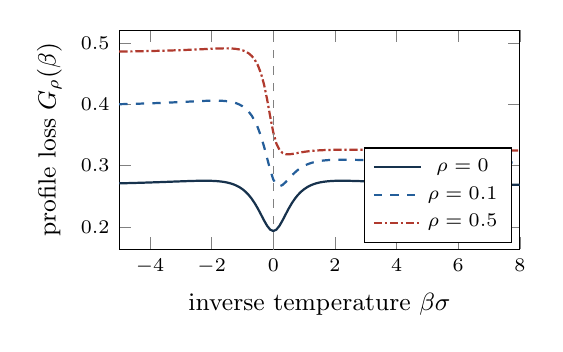
\begin{tikzpicture}
\begin{axis}[width=0.55\textwidth,height=0.36\textwidth,xmin=-5,xmax=8,xlabel={inverse temperature $\beta\sigma$},ylabel={profile loss $G_\rho(\beta)$},
  tick label style={font=\scriptsize},label style={font=\small},
  legend style={font=\scriptsize,at={(0.98,0.03)},anchor=south east}]
\addplot[no marks,thick,color=Navy] coordinates {(-5.0,0.270946) (-4.9,0.271070) (-4.8,0.271198) (-4.7,0.271330) (-4.6,0.271467) (-4.5,0.271608) (-4.4,0.271755) (-4.3,0.271906) (-4.2,0.272062) (-4.1,0.272223) (-4.0,0.272389) (-3.9,0.272559) (-3.8,0.272734) (-3.7,0.272913) (-3.6,0.273097) (-3.5,0.273283) (-3.4,0.273473) (-3.3,0.273664) (-3.2,0.273855) (-3.1,0.274046) (-3.0,0.274235) (-2.9,0.274418) (-2.8,0.274594) (-2.7,0.274758) (-2.6,0.274907) (-2.5,0.275033) (-2.4,0.275131) (-2.3,0.275192) (-2.2,0.275205) (-2.1,0.275157) (-2.0,0.275030) (-1.9,0.274806) (-1.8,0.274457) (-1.7,0.273954) (-1.6,0.273255) (-1.5,0.272315) (-1.4,0.271072) (-1.3,0.269455) (-1.2,0.267376) (-1.1,0.264728) (-1.0,0.261389) (-0.9,0.257218) (-0.8,0.252067) (-0.7,0.245799) (-0.6,0.238328) (-0.5,0.229687) (-0.4,0.220148) (-0.3,0.210382) (-0.2,0.201580) (-0.1,0.195338) (-0.0,0.193075) (0.1,0.195338) (0.2,0.201580) (0.3,0.210382) (0.4,0.220148) (0.5,0.229687) (0.6,0.238328) (0.7,0.245799) (0.8,0.252067) (0.9,0.257218) (1.0,0.261389) (1.1,0.264728) (1.2,0.267376) (1.3,0.269455) (1.4,0.271072) (1.5,0.272315) (1.6,0.273255) (1.7,0.273954) (1.8,0.274457) (1.9,0.274806) (2.0,0.275030) (2.1,0.275157) (2.2,0.275205) (2.3,0.275192) (2.4,0.275131) (2.5,0.275033) (2.6,0.274907) (2.7,0.274758) (2.8,0.274594) (2.9,0.274418) (3.0,0.274235) (3.1,0.274046) (3.2,0.273855) (3.3,0.273664) (3.4,0.273473) (3.5,0.273283) (3.6,0.273097) (3.7,0.272913) (3.8,0.272734) (3.9,0.272559) (4.0,0.272389) (4.1,0.272223) (4.2,0.272062) (4.3,0.271906) (4.4,0.271755) (4.5,0.271608) (4.6,0.271467) (4.7,0.271330) (4.8,0.271198) (4.9,0.271070) (5.0,0.270946) (5.1,0.270827) (5.2,0.270712) (5.3,0.270601) (5.4,0.270494) (5.5,0.270390) (5.6,0.270290) (5.7,0.270194) (5.8,0.270100) (5.9,0.270010) (6.0,0.269923) (6.1,0.269839) (6.2,0.269758) (6.3,0.269679) (6.4,0.269604) (6.5,0.269530) (6.6,0.269459) (6.7,0.269391) (6.8,0.269324) (6.9,0.269260) (7.0,0.269198) (7.1,0.269137) (7.2,0.269079) (7.3,0.269023) (7.4,0.268968) (7.5,0.268915) (7.6,0.268863) (7.7,0.268813) (7.8,0.268765) (7.9,0.268718) (8.0,0.268673)};
\addlegendentry{$\rho=0$}
\addplot[no marks,thick,color=Blue,dashed] coordinates {(-5.0,0.400242) (-4.9,0.400360) (-4.8,0.400483) (-4.7,0.400611) (-4.6,0.400745) (-4.5,0.400885) (-4.4,0.401030) (-4.3,0.401181) (-4.2,0.401339) (-4.1,0.401504) (-4.0,0.401676) (-3.9,0.401854) (-3.8,0.402040) (-3.7,0.402234) (-3.6,0.402435) (-3.5,0.402643) (-3.4,0.402859) (-3.3,0.403083) (-3.2,0.403313) (-3.1,0.403551) (-3.0,0.403794) (-2.9,0.404042) (-2.8,0.404293) (-2.7,0.404545) (-2.6,0.404796) (-2.5,0.405043) (-2.4,0.405280) (-2.3,0.405502) (-2.2,0.405701) (-2.1,0.405867) (-2.0,0.405988) (-1.9,0.406046) (-1.8,0.406020) (-1.7,0.405882) (-1.6,0.405597) (-1.5,0.405117) (-1.4,0.404382) (-1.3,0.403313) (-1.2,0.401809) (-1.1,0.399736) (-1.0,0.396921) (-0.9,0.393144) (-0.8,0.388123) (-0.7,0.381506) (-0.6,0.372880) (-0.5,0.361797) (-0.4,0.347880) (-0.3,0.331056) (-0.2,0.312023) (-0.1,0.292892) (-0.0,0.277313) (0.1,0.268401) (0.2,0.266100) (0.3,0.268319) (0.4,0.272912) (0.5,0.278357) (0.6,0.283761) (0.7,0.288681) (0.8,0.292945) (0.9,0.296526) (1.0,0.299473) (1.1,0.301861) (1.2,0.303772) (1.3,0.305285) (1.4,0.306471) (1.5,0.307388) (1.6,0.308087) (1.7,0.308610) (1.8,0.308992) (1.9,0.309259) (2.0,0.309436) (2.1,0.309539) (2.2,0.309585) (2.3,0.309585) (2.4,0.309549) (2.5,0.309485) (2.6,0.309400) (2.7,0.309297) (2.8,0.309183) (2.9,0.309060) (3.0,0.308930) (3.1,0.308796) (3.2,0.308660) (3.3,0.308523) (3.4,0.308386) (3.5,0.308250) (3.6,0.308116) (3.7,0.307984) (3.8,0.307855) (3.9,0.307728) (4.0,0.307605) (4.1,0.307485) (4.2,0.307368) (4.3,0.307255) (4.4,0.307145) (4.5,0.307039) (4.6,0.306936) (4.7,0.306836) (4.8,0.306740) (4.9,0.306647) (5.0,0.306557) (5.1,0.306470) (5.2,0.306386) (5.3,0.306305) (5.4,0.306226) (5.5,0.306151) (5.6,0.306077) (5.7,0.306007) (5.8,0.305938) (5.9,0.305872) (6.0,0.305809) (6.1,0.305747) (6.2,0.305687) (6.3,0.305630) (6.4,0.305574) (6.5,0.305520) (6.6,0.305468) (6.7,0.305417) (6.8,0.305369) (6.9,0.305321) (7.0,0.305276) (7.1,0.305231) (7.2,0.305188) (7.3,0.305147) (7.4,0.305106) (7.5,0.305067) (7.6,0.305029) (7.7,0.304993) (7.8,0.304957) (7.9,0.304922) (8.0,0.304889)};
\addlegendentry{$\rho=0.1$}
\addplot[no marks,thick,color=Red,densely dashdotted] coordinates {(-5.0,0.486235) (-4.9,0.486305) (-4.8,0.486378) (-4.7,0.486455) (-4.6,0.486536) (-4.5,0.486621) (-4.4,0.486710) (-4.3,0.486804) (-4.2,0.486903) (-4.1,0.487007) (-4.0,0.487117) (-3.9,0.487232) (-3.8,0.487354) (-3.7,0.487482) (-3.6,0.487617) (-3.5,0.487760) (-3.4,0.487909) (-3.3,0.488067) (-3.2,0.488233) (-3.1,0.488408) (-3.0,0.488591) (-2.9,0.488784) (-2.8,0.488985) (-2.7,0.489194) (-2.6,0.489413) (-2.5,0.489638) (-2.4,0.489870) (-2.3,0.490106) (-2.2,0.490344) (-2.1,0.490579) (-2.0,0.490807) (-1.9,0.491020) (-1.8,0.491208) (-1.7,0.491356) (-1.6,0.491446) (-1.5,0.491451) (-1.4,0.491335) (-1.3,0.491048) (-1.2,0.490521) (-1.1,0.489659) (-1.0,0.488324) (-0.9,0.486324) (-0.8,0.483377) (-0.7,0.479075) (-0.6,0.472820) (-0.5,0.463752) (-0.4,0.450702) (-0.3,0.432361) (-0.2,0.408111) (-0.1,0.380027) (-0.0,0.354188) (0.1,0.336063) (0.2,0.325697) (0.3,0.320625) (0.4,0.318659) (0.5,0.318358) (0.6,0.318872) (0.7,0.319726) (0.8,0.320668) (0.9,0.321573) (1.0,0.322387) (1.1,0.323091) (1.2,0.323685) (1.3,0.324177) (1.4,0.324579) (1.5,0.324904) (1.6,0.325164) (1.7,0.325368) (1.8,0.325527) (1.9,0.325649) (2.0,0.325739) (2.1,0.325804) (2.2,0.325848) (2.3,0.325875) (2.4,0.325888) (2.5,0.325890) (2.6,0.325883) (2.7,0.325868) (2.8,0.325848) (2.9,0.325823) (3.0,0.325795) (3.1,0.325764) (3.2,0.325731) (3.3,0.325696) (3.4,0.325661) (3.5,0.325625) (3.6,0.325588) (3.7,0.325552) (3.8,0.325515) (3.9,0.325479) (4.0,0.325443) (4.1,0.325408) (4.2,0.325374) (4.3,0.325340) (4.4,0.325307) (4.5,0.325274) (4.6,0.325243) (4.7,0.325212) (4.8,0.325182) (4.9,0.325153) (5.0,0.325124) (5.1,0.325097) (5.2,0.325070) (5.3,0.325044) (5.4,0.325018) (5.5,0.324994) (5.6,0.324970) (5.7,0.324947) (5.8,0.324924) (5.9,0.324903) (6.0,0.324881) (6.1,0.324861) (6.2,0.324841) (6.3,0.324822) (6.4,0.324803) (6.5,0.324785) (6.6,0.324767) (6.7,0.324750) (6.8,0.324733) (6.9,0.324717) (7.0,0.324702) (7.1,0.324686) (7.2,0.324672) (7.3,0.324657) (7.4,0.324643) (7.5,0.324630) (7.6,0.324617) (7.7,0.324604) (7.8,0.324591) (7.9,0.324579) (8.0,0.324567)};
\addlegendentry{$\rho=0.5$}

\draw[gray,dashed] (axis cs:0,0.15) -- (axis cs:0,0.52);
\end{axis}
\end{tikzpicture}
\caption{Profile loss $G_\rho(\beta)=\min_{u,c}L(\beta,u,c;\rho)$ for $k=2$ and $\delta/\sigma=2$, computed by Gauss--Hermite quadrature in $\bar a$ and a fine grid in $a_1-a_2$. Without near-misses ($\rho=0$) the minimum is the SUM; with near-misses it moves to a soft AND $\beta^\star>0$. Local maxima separate the soft AND from the OR at $\beta=-\infty$ and, for $\rho\in\{0,0.5\}$, from the hard AND at $\beta=+\infty$.}\label{fig:landscape}
\end{figure}

%% ----------------------------------------------------------------------
\section{Implementation Details}\label{app:expdetails}

All models are implemented in NumPy with analytic gradients, which were checked against finite differences. Synthetic windows have 20 sensors and 48 time steps. Every sensor carries AR(1) Gaussian noise with coefficient 0.7, six sensors share a slow common load, and Fault~1 lowers three sensors by $2.5\sigma$ from a random onset. The look-alikes are built from the same step change: the one-of-three and two-of-three look-alikes shift one or two of the three sensors, and the loud look-alike shifts a single sensor by three times the fault amount.

The fan-coil data are the one-year simulations of a fan-coil unit in the LBNL dataset \citep{granderson2023}, which consist of one fault-free run and runs with individual faults under the same building and weather. The target fault is \texttt{FCU\_FanOutletBlockage}, whose signature sensors \texttt{FCU\_CLG\_GPM} (cooling-water flow), \texttt{FCU\_CVLV} (cooling-valve position) and \texttt{FCU\_WAT} (a third water-side point) shift by 2.6, 2.3 and 1.7 standard deviations. After the removal of label columns and of channels that are constant in fault-free data, 24 sensors remain; the data are resampled to 15 minutes and cut into windows of 48 steps (12 hours). Because the runs are paired, the effect of the fault on each sensor and time step is $\Delta X=X^{\mathrm{fault}}-X^{\mathrm{normal}}$, and windows are built by counterfactual splicing $X=W+M\odot\Delta X$, where $W$ is a fault-free window and the mask $M$ selects the sensors and time steps that receive the fault effect. A near-miss of type $j$ uses the mask of Fault~1 with sensor $j$ removed, and the look-alikes are built in the same way.

The transformer embeds each sensor's 48-step series with a two-layer MLP (width 32, ReLU), adds a learned sensor embedding, applies one self-attention layer with a residual connection \citep{vaswani2017}, and pools the tokens by softmax attention with a learned query, followed by a linear head. The attention pool is the same model without the self-attention layer, that is, the model of \cref{thm:attn,thm:soft} with the evidence replaced by a learned embedding. Training uses Adam \citep{kingma2015} with learning rate $3\times10^{-3}$, batch size 64, at most 30 epochs, early stopping on a 15\% validation split with patience 6, the logistic loss and gradient clipping at 5. The plain training set has 4{,}000 normal and Fault~1 windows, and the +NM set adds 2{,}000 near-misses, split over the three types. The alarm threshold gives 1\% false alarms on held-out normal windows, and every look-alike is tested on 1{,}000 windows with seeds 0, 1 and 2.

The learned inverse temperature of the attention pool is read from its attention weights. In the reduced model, $\log\pi_j=-\beta a_j+\mathrm{const}$ within a window, so $\hat\beta$ is minus the pooled within-window slope of $\log\pi_j$ on the per-sensor evidence $a_j$ over the signature sensors, computed on Fault~1 and near-miss test windows. A value $\hat\beta>0$ places more weight on the sensor with less evidence (AND-like), and $\hat\beta<0$ on the sensor with more evidence (OR-like). The left-out ratio is the attention on the unshifted sensor of a near-miss window divided by the mean attention on the other signature sensors.

%% ----------------------------------------------------------------------
\section{Full Experimental Results}\label{app:results}

All entries are fractions of windows that raise an alarm at 1\% false alarms on normal windows, averaged over three seeds; standard deviations are in the repository reports. The AND rule is the oracle that thresholds the minimum of the true per-sensor shifts.

\begin{table}[h]\centering\small\setlength{\tabcolsep}{3.5pt}
\renewcommand{\arraystretch}{1.15}
\caption{Synthetic data. \emph{law}: the two-of-three rate predicted by \cref{thm:sum}(ii) from the model's own detection rate. Under +NM, the one-of-three and loud look-alikes were never used in training.}\label{tab:toy}
\begin{tabular}{@{}lccccc|cccc@{}}\toprule
 & \multicolumn{5}{c|}{\emph{plain} (normal vs.\ Fault~1)} & \multicolumn{4}{c}{\emph{+NM} (+ near-misses)}\\
Model & Fault 1 & 1-of-3 & 2-of-3 & law & loud one & Fault 1 & 1-of-3 & 2-of-3 & loud one\\\midrule
Transformer (sensor tokens) & 0.93 & 0.45 & 0.78 & 0.59 & 1.00 & 0.88 & 0.03 & 0.15 & 0.02\\
Attention pool & 0.91 & 0.48 & 0.79 & 0.56 & 1.00 & 0.84 & 0.03 & 0.11 & 0.02\\
\midrule
AND rule (oracle) & 0.90 & 0.06 & 0.22 & -- & 0.06 & 0.88 & 0.05 & 0.20 & 0.05\\
\bottomrule\end{tabular}\end{table}

After plain training both models lie about 0.2 above the law of \cref{thm:sum}(ii) at their own detection rate and flag the loud single sensor in every window. This is the OR-like score that \cref{thm:attn}(c) predicts with 17 irrelevant sensors, and \cref{tab:focus} confirms it with $\hat\beta<0$. With near-misses both models fall to 0.11--0.15 on two-of-three look-alikes, at or below the oracle, and to 0.02--0.03 on the one-of-three and loud look-alikes, neither of which appears in training. A detector that is monotone in the set of shifted sensors and rejects the $k$ near-misses rejects every partial look-alike, since each partial look-alike shifts a subset of the sensors of some near-miss, and an AND also rejects loud look-alikes (\cref{thm:and}(b)).

\begin{table}[h]\centering\small
\renewcommand{\arraystretch}{1.15}
\caption{Learned attention of the attention-pool model (mean\,$\pm$\,s.d.\ over 3 seeds). $\hat\beta$: learned inverse temperature; left-out ratio: attention on the unshifted sensor of a two-of-three window relative to the other signature sensors; mass: total attention on the signature sensors. On fan-coil with near-misses the left-out ratio varies over orders of magnitude between seeds, so its minimum is reported.}\label{tab:focus}
\begin{tabular}{@{}lccc|ccc@{}}\toprule
 & \multicolumn{3}{c|}{synthetic} & \multicolumn{3}{c}{LBNL fan-coil}\\
Training set & $\hat\beta$ & left-out ratio & mass & $\hat\beta$ & left-out ratio & mass\\\midrule
\emph{plain} & $-$1.06\,{\scriptsize$\pm$0.23} & 0.14\,{\scriptsize$\pm$0.04} & 0.83\,{\scriptsize$\pm$0.03} & $-$1.02\,{\scriptsize$\pm$0.21} & 0.01\,{\scriptsize$\pm$0.01} & 0.98\,{\scriptsize$\pm$0.00}\\
\emph{+NM} & 0.70\,{\scriptsize$\pm$0.11} & 10.63\,{\scriptsize$\pm$3.89} & 0.96\,{\scriptsize$\pm$0.02} & 0.69\,{\scriptsize$\pm$0.17} & $\ge$88 (min) & 0.74\,{\scriptsize$\pm$0.15}\\
\bottomrule\end{tabular}

\end{table}

\begin{figure}[h]\centering
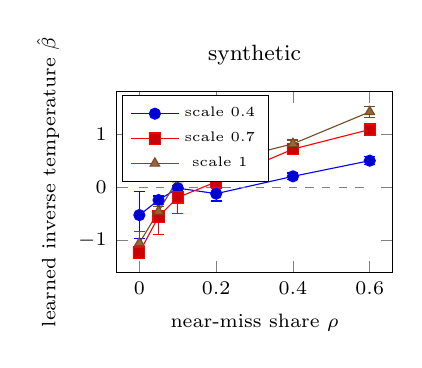
\begin{tikzpicture}
\begin{axis}[width=0.42\linewidth,height=0.32\linewidth,xlabel={near-miss share $\rho$},title={synthetic},title style={font=\footnotesize},tick label style={font=\scriptsize},label style={font=\scriptsize},legend style={font=\tiny,at={(0.02,0.98)},anchor=north west},ylabel={learned inverse temperature $\hat\beta$}]
\addplot+[mark=*,error bars/.cd,y dir=both,y explicit] coordinates {(0,-0.522) +- (0,0.447) (0.05,-0.237) +- (0,0.076) (0.1,-0.011) +- (0,0.058) (0.2,-0.116) +- (0,0.139) (0.4,0.212) +- (0,0.064) (0.6,0.509) +- (0,0.075)};\addlegendentry{scale 0.4}
\addplot+[mark=square*,error bars/.cd,y dir=both,y explicit] coordinates {(0,-1.231) +- (0,0.094) (0.05,-0.550) +- (0,0.343) (0.1,-0.188) +- (0,0.309) (0.2,0.107) +- (0,0.123) (0.4,0.728) +- (0,0.079) (0.6,1.099) +- (0,0.111)};\addlegendentry{scale 0.7}
\addplot+[mark=triangle*,error bars/.cd,y dir=both,y explicit] coordinates {(0,-1.051) +- (0,0.211) (0.05,-0.451) +- (0,0.097) (0.1,0.159) +- (0,0.175) (0.2,0.462) +- (0,0.047) (0.4,0.828) +- (0,0.073) (0.6,1.433) +- (0,0.099)};\addlegendentry{scale 1}
\addplot[gray,dashed,domain=0:0.6]{0};
\end{axis}
\end{tikzpicture}\hspace{8mm}
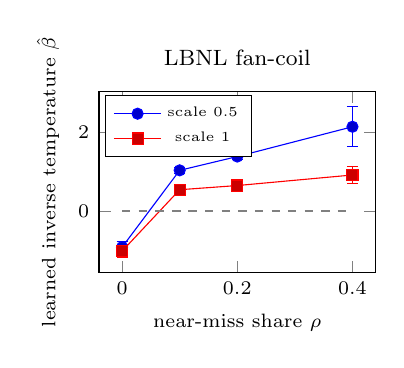
\begin{tikzpicture}
\begin{axis}[width=0.42\linewidth,height=0.32\linewidth,xlabel={near-miss share $\rho$},title={LBNL fan-coil},title style={font=\footnotesize},tick label style={font=\scriptsize},label style={font=\scriptsize},legend style={font=\tiny,at={(0.02,0.98)},anchor=north west},ylabel={learned inverse temperature $\hat\beta$}]
\addplot+[mark=*,error bars/.cd,y dir=both,y explicit] coordinates {(0,-0.917) +- (0,0.150) (0.1,1.033) +- (0,0.069) (0.2,1.383) +- (0,0.086) (0.4,2.139) +- (0,0.510)};\addlegendentry{scale 0.5}
\addplot+[mark=square*,error bars/.cd,y dir=both,y explicit] coordinates {(0,-1.018) +- (0,0.161) (0.1,0.541) +- (0,0.103) (0.2,0.647) +- (0,0.106) (0.4,0.915) +- (0,0.218)};\addlegendentry{scale 1}
\addplot[gray,dashed,domain=0:0.4]{0};
\end{axis}
\end{tikzpicture}
\caption{Soft AND in a trained model (attention pool, mean over 3 seeds, bars: s.d.). The learned inverse temperature is finite and increases with the near-miss share $\rho$, as \cref{thm:soft} predicts; on synthetic data it also increases with the fault scale from $\rho=0.2$ on. It starts negative because of the OR push of the irrelevant sensors (\cref{thm:attn}(c)). On fan-coil both scales lie far from the noisy regime of \cref{thm:soft} (detection at least 0.97 at scale 0.5), and since $\hat\beta$ is a slope per unit of evidence, halving the shift doubles the $\hat\beta$ needed for the same contrast. Alarms on two-of-three look-alikes fall from 0.78 to 0.12 (synthetic, scale 1, $\rho=0.2$) and from 0.98 to 0.12 (fan-coil, $\rho=0.4$).}\label{fig:softand}
\end{figure}

\begin{table}[h]\centering\small\setlength{\tabcolsep}{3pt}
\renewcommand{\arraystretch}{1.15}
\caption{Synthetic data, \emph{plain} training: look-alikes flagged as their shift grows to $M$ times Fault~1's.}\label{tab:strength}
\begin{tabular}{@{}lcccccc|cccccc@{}}\toprule
 & \multicolumn{6}{c|}{two-of-three look-alike, strength $M$} & \multicolumn{6}{c}{one-sensor look-alike, strength $M$}\\
Model & 0.5 & 1 & 1.5 & 2 & 3 & 5 & 0.5 & 1 & 1.5 & 2 & 3 & 5\\\midrule
Transformer (sensor tokens) & 0.19 & 0.77 & 0.99 & 1.00 & 1.00 & 1.00 & 0.08 & 0.43 & 0.86 & 0.99 & 1.00 & 1.00\\
Attention pool & 0.16 & 0.78 & 1.00 & 1.00 & 1.00 & 1.00 & 0.08 & 0.42 & 0.89 & 0.99 & 1.00 & 1.00\\
\bottomrule\end{tabular}\end{table}

\Cref{thm:and}(c,d) predicts that detectors whose score grows without bound in each sensor flag look-alikes more often as the look-alikes become louder. After plain training both models flag two-of-three look-alikes in at least 0.99 of windows from $M=1.5$ and one-sensor look-alikes from $M=2$ (\cref{tab:strength}). After near-misses the attention pool is flat in $M$, with 0.07--0.12 on two-of-three look-alikes for $M$ between 1 and 5, as expected of a score that computes an AND.

\begin{table}[h]\centering\small\setlength{\tabcolsep}{3.5pt}
\renewcommand{\arraystretch}{1.15}
\caption{LBNL fan-coil unit, Fault~1 = \texttt{FCU\_FanOutletBlockage}; columns as in \cref{tab:toy}.}\label{tab:fcu}
\begin{tabular}{@{}lccccc|cccc@{}}\toprule
 & \multicolumn{5}{c|}{\emph{plain}} & \multicolumn{4}{c}{\emph{+NM}}\\
Model & Fault 1 & 1-of-3 & 2-of-3 & law & loud one & Fault 1 & 1-of-3 & 2-of-3 & loud one\\\midrule
Transformer (sensor tokens) & 1.00 & 0.96 & 0.99 & 0.96 & 1.00 & 1.00 & 0.06 & 0.18 & 0.05\\
Attention pool & 1.00 & 0.90 & 0.98 & 0.93 & 1.00 & 1.00 & 0.03 & 0.20 & 0.02\\
\midrule
AND rule (oracle) & 1.00 & 0.08 & 0.33 & -- & 0.07 & 1.00 & 0.07 & 0.31 & 0.06\\
\bottomrule\end{tabular}\end{table}

On the fan-coil unit detection saturates at 1.00, so the law predicts that almost every two-of-three look-alike is flagged (0.93--0.96), and after plain training the models flag 0.98--0.99 against 0.33 for the oracle (\cref{tab:fcu}). With detection at 1.00 the law cannot distinguish an additive score from an OR-like one, but the learned attention can: without near-misses $\hat\beta=-1.02$ and the unshifted sensor of a two-of-three window receives 0.01 of the weight of the others, whereas with near-misses $\hat\beta=0.69$ and it receives at least 88 times their weight. After near-misses the transformer flags two-of-three look-alikes in 0.18 of windows and the attention pool in 0.20 (oracle 0.31), and the one-sensor and loud look-alikes fall to 0.02--0.06.

\FloatBarrier
%% ----------------------------------------------------------------------
\section{Reproducibility}\label{app:repro}

The code is available at \url{https://github.com/chirag300/HVAC_Test} (tag \texttt{cs886-final}), whose README lists the directory layout and the reproduction steps. It requires Python 3 with NumPy, pandas, scikit-learn and matplotlib (\texttt{requirements.txt}), and the theory checks also use SciPy; no GPU or deep-learning framework is needed. Reference outputs for both datasets are stored in \texttt{reference\_results/transformer\_toy} and \texttt{reference\_results/transformer\_fcu}, with a report, JSON files for every cell and seed, and figures. The script \texttt{verify\_all.py} in the repository compares every closed-form expression with a direct computation by Monte Carlo with $10^6$ to $4\times10^6$ samples, Gauss--Hermite quadrature or brute-force optimisation; all 53 checks pass within Monte Carlo error. The LBNL dataset \citep{granderson2023} is public and is fetched by \texttt{python download.py fcu}; the synthetic source needs no data. The results are reproduced by the following commands.
{\small
\begin{verbatim}
pip install -r requirements.txt
python transformer_numpy.py          # gradient checks of all models -> PASS
python theory/attention_checks.py    # repository checks of Theorems 3-4 (~5 min)
python verify_all.py                 # independent checks of every formula (~6 min)
python run_transformer.py --out results/transformer_toy --seeds 0,1,2     # ~1.5 h
python run_transformer.py --data data/raw/fcu --out results/transformer_fcu \
    --target FCU_FanOutletBlockage --seeds 0,1,2 --rhos 0,0.1,0.2,0.4 \
    --snr-scales 0.5,1
\end{verbatim}}
\noindent Every cell is cached as JSON, and interrupted runs resume. The defaults are \texttt{--n-train 4000}, \texttt{--n-test 1000} and \texttt{--epochs 30}, with strengths $\{0.5,1,1.5,2,3,5\}$, synthetic near-miss shares $\{0,0.05,0.1,0.2,0.4,0.6\}$ and fault scales $\{0.4,0.7,1\}$. All results were produced on CPU; the synthetic battery takes about 1.5 hours on two cores, and the numerical checks take a few minutes.


\end{document}
